% Options for packages loaded elsewhere
\PassOptionsToPackage{unicode}{hyperref}
\PassOptionsToPackage{hyphens}{url}
%
\documentclass[
]{book}
\usepackage{lmodern}
\usepackage{amssymb,amsmath}
\usepackage{ifxetex,ifluatex}
\ifnum 0\ifxetex 1\fi\ifluatex 1\fi=0 % if pdftex
  \usepackage[T1]{fontenc}
  \usepackage[utf8]{inputenc}
  \usepackage{textcomp} % provide euro and other symbols
\else % if luatex or xetex
  \usepackage{unicode-math}
  \defaultfontfeatures{Scale=MatchLowercase}
  \defaultfontfeatures[\rmfamily]{Ligatures=TeX,Scale=1}
\fi
% Use upquote if available, for straight quotes in verbatim environments
\IfFileExists{upquote.sty}{\usepackage{upquote}}{}
\IfFileExists{microtype.sty}{% use microtype if available
  \usepackage[]{microtype}
  \UseMicrotypeSet[protrusion]{basicmath} % disable protrusion for tt fonts
}{}
\makeatletter
\@ifundefined{KOMAClassName}{% if non-KOMA class
  \IfFileExists{parskip.sty}{%
    \usepackage{parskip}
  }{% else
    \setlength{\parindent}{0pt}
    \setlength{\parskip}{6pt plus 2pt minus 1pt}}
}{% if KOMA class
  \KOMAoptions{parskip=half}}
\makeatother
\usepackage{xcolor}
\IfFileExists{xurl.sty}{\usepackage{xurl}}{} % add URL line breaks if available
\IfFileExists{bookmark.sty}{\usepackage{bookmark}}{\usepackage{hyperref}}
\hypersetup{
  pdftitle={Técnicas cuantitativas},
  pdfauthor={Enric Aguilar y Benito Zaragozí},
  hidelinks,
  pdfcreator={LaTeX via pandoc}}
\urlstyle{same} % disable monospaced font for URLs
\usepackage{color}
\usepackage{fancyvrb}
\newcommand{\VerbBar}{|}
\newcommand{\VERB}{\Verb[commandchars=\\\{\}]}
\DefineVerbatimEnvironment{Highlighting}{Verbatim}{commandchars=\\\{\}}
% Add ',fontsize=\small' for more characters per line
\usepackage{framed}
\definecolor{shadecolor}{RGB}{248,248,248}
\newenvironment{Shaded}{\begin{snugshade}}{\end{snugshade}}
\newcommand{\AlertTok}[1]{\textcolor[rgb]{0.94,0.16,0.16}{#1}}
\newcommand{\AnnotationTok}[1]{\textcolor[rgb]{0.56,0.35,0.01}{\textbf{\textit{#1}}}}
\newcommand{\AttributeTok}[1]{\textcolor[rgb]{0.77,0.63,0.00}{#1}}
\newcommand{\BaseNTok}[1]{\textcolor[rgb]{0.00,0.00,0.81}{#1}}
\newcommand{\BuiltInTok}[1]{#1}
\newcommand{\CharTok}[1]{\textcolor[rgb]{0.31,0.60,0.02}{#1}}
\newcommand{\CommentTok}[1]{\textcolor[rgb]{0.56,0.35,0.01}{\textit{#1}}}
\newcommand{\CommentVarTok}[1]{\textcolor[rgb]{0.56,0.35,0.01}{\textbf{\textit{#1}}}}
\newcommand{\ConstantTok}[1]{\textcolor[rgb]{0.00,0.00,0.00}{#1}}
\newcommand{\ControlFlowTok}[1]{\textcolor[rgb]{0.13,0.29,0.53}{\textbf{#1}}}
\newcommand{\DataTypeTok}[1]{\textcolor[rgb]{0.13,0.29,0.53}{#1}}
\newcommand{\DecValTok}[1]{\textcolor[rgb]{0.00,0.00,0.81}{#1}}
\newcommand{\DocumentationTok}[1]{\textcolor[rgb]{0.56,0.35,0.01}{\textbf{\textit{#1}}}}
\newcommand{\ErrorTok}[1]{\textcolor[rgb]{0.64,0.00,0.00}{\textbf{#1}}}
\newcommand{\ExtensionTok}[1]{#1}
\newcommand{\FloatTok}[1]{\textcolor[rgb]{0.00,0.00,0.81}{#1}}
\newcommand{\FunctionTok}[1]{\textcolor[rgb]{0.00,0.00,0.00}{#1}}
\newcommand{\ImportTok}[1]{#1}
\newcommand{\InformationTok}[1]{\textcolor[rgb]{0.56,0.35,0.01}{\textbf{\textit{#1}}}}
\newcommand{\KeywordTok}[1]{\textcolor[rgb]{0.13,0.29,0.53}{\textbf{#1}}}
\newcommand{\NormalTok}[1]{#1}
\newcommand{\OperatorTok}[1]{\textcolor[rgb]{0.81,0.36,0.00}{\textbf{#1}}}
\newcommand{\OtherTok}[1]{\textcolor[rgb]{0.56,0.35,0.01}{#1}}
\newcommand{\PreprocessorTok}[1]{\textcolor[rgb]{0.56,0.35,0.01}{\textit{#1}}}
\newcommand{\RegionMarkerTok}[1]{#1}
\newcommand{\SpecialCharTok}[1]{\textcolor[rgb]{0.00,0.00,0.00}{#1}}
\newcommand{\SpecialStringTok}[1]{\textcolor[rgb]{0.31,0.60,0.02}{#1}}
\newcommand{\StringTok}[1]{\textcolor[rgb]{0.31,0.60,0.02}{#1}}
\newcommand{\VariableTok}[1]{\textcolor[rgb]{0.00,0.00,0.00}{#1}}
\newcommand{\VerbatimStringTok}[1]{\textcolor[rgb]{0.31,0.60,0.02}{#1}}
\newcommand{\WarningTok}[1]{\textcolor[rgb]{0.56,0.35,0.01}{\textbf{\textit{#1}}}}
\usepackage{longtable,booktabs}
% Correct order of tables after \paragraph or \subparagraph
\usepackage{etoolbox}
\makeatletter
\patchcmd\longtable{\par}{\if@noskipsec\mbox{}\fi\par}{}{}
\makeatother
% Allow footnotes in longtable head/foot
\IfFileExists{footnotehyper.sty}{\usepackage{footnotehyper}}{\usepackage{footnote}}
\makesavenoteenv{longtable}
\usepackage{graphicx,grffile}
\makeatletter
\def\maxwidth{\ifdim\Gin@nat@width>\linewidth\linewidth\else\Gin@nat@width\fi}
\def\maxheight{\ifdim\Gin@nat@height>\textheight\textheight\else\Gin@nat@height\fi}
\makeatother
% Scale images if necessary, so that they will not overflow the page
% margins by default, and it is still possible to overwrite the defaults
% using explicit options in \includegraphics[width, height, ...]{}
\setkeys{Gin}{width=\maxwidth,height=\maxheight,keepaspectratio}
% Set default figure placement to htbp
\makeatletter
\def\fps@figure{htbp}
\makeatother
\setlength{\emergencystretch}{3em} % prevent overfull lines
\providecommand{\tightlist}{%
  \setlength{\itemsep}{0pt}\setlength{\parskip}{0pt}}
\setcounter{secnumdepth}{5}
\usepackage{booktabs}

\ifxetex
  \usepackage{polyglossia}
  \setmainlanguage{spanish}
  % Tabla en lugar de cuadro
  \gappto\captionsspanish{\renewcommand{\tablename}{Tabla}  
          \renewcommand{\listtablename}{Índice de tablas}}
\else
  \usepackage[spanish,es-tabla]{babel}
\fi
\usepackage{booktabs}
\usepackage{longtable}
\usepackage{array}
\usepackage{multirow}
\usepackage{wrapfig}
\usepackage{float}
\usepackage{colortbl}
\usepackage{pdflscape}
\usepackage{tabu}
\usepackage{threeparttable}
\usepackage{threeparttablex}
\usepackage[normalem]{ulem}
\usepackage{makecell}
\usepackage{xcolor}
\usepackage[]{natbib}
\bibliographystyle{apalike}

\title{Técnicas cuantitativas}
\author{Enric Aguilar y Benito Zaragozí}
\date{06-Apr-2021}

\begin{document}
\maketitle

{
\setcounter{tocdepth}{1}
\tableofcontents
}
\hypertarget{antes-de-empezar}{%
\chapter*{Antes de empezar}\label{antes-de-empezar}}
\addcontentsline{toc}{chapter}{Antes de empezar}

En este breve capítulo explicamos los aspectos básicos para que podáis reproducir los ejercicios y entregar las actividades utilizando R, Markdown y Rstudio. Aquí planteamos los conceptos básicos para preparar un documento que incluye explicaciónes, código y los resultados de análisis R. Se trata de una estratégia de \textbf{\emph{programación literaria}} que en los últimos años está siendo cada vez más utilizada en el análisis de datos \citep{knuth1984literate, xie2015knitr}.

\hypertarget{prerrequisitos}{%
\section{Prerrequisitos}\label{prerrequisitos}}

Para seguir las explicaciones de este curso será necesario instalar primero R y RStudio con los paquetes \texttt{knitr} y \texttt{rmarkdown}. A continuación mostramos la configuración general del sistema R utilizado.

\begin{Shaded}
\begin{Highlighting}[]
\KeywordTok{sessionInfo}\NormalTok{()}
\end{Highlighting}
\end{Shaded}

\begin{verbatim}
## R version 4.0.2 (2020-06-22)
## Platform: x86_64-pc-linux-gnu (64-bit)
## Running under: Ubuntu 20.04 LTS
## 
## Matrix products: default
## BLAS/LAPACK: /usr/lib/x86_64-linux-gnu/openblas-pthread/libopenblasp-r0.3.8.so
## 
## locale:
##  [1] LC_CTYPE=en_US.UTF-8       LC_NUMERIC=C              
##  [3] LC_TIME=en_US.UTF-8        LC_COLLATE=en_US.UTF-8    
##  [5] LC_MONETARY=en_US.UTF-8    LC_MESSAGES=C             
##  [7] LC_PAPER=en_US.UTF-8       LC_NAME=C                 
##  [9] LC_ADDRESS=C               LC_TELEPHONE=C            
## [11] LC_MEASUREMENT=en_US.UTF-8 LC_IDENTIFICATION=C       
## 
## attached base packages:
## [1] stats     graphics  grDevices utils     datasets  methods   base     
## 
## other attached packages:
## [1] pander_0.6.3
## 
## loaded via a namespace (and not attached):
##  [1] compiler_4.0.2  magrittr_1.5    bookdown_0.21   htmltools_0.5.0
##  [5] tools_4.0.2     rstudioapi_0.11 yaml_2.2.1      Rcpp_1.0.5     
##  [9] stringi_1.5.3   rmarkdown_2.4   knitr_1.30      stringr_1.4.0  
## [13] digest_0.6.25   xfun_0.22       rlang_0.4.7     evaluate_0.14
\end{verbatim}

\hypertarget{tipos-de-ficheros}{%
\section{Tipos de ficheros}\label{tipos-de-ficheros}}

\begin{itemize}
\tightlist
\item
  Los archivos para producir documentos de RMarkdown tienen la extensión \texttt{.Rmd}.
\item
  Los archivos deben abrirse con RStudio y se compilan haciendo clic en el botón knitr.
\item
  El resultado es un documento en formato \texttt{.pdf}, \texttt{.html} o \texttt{.doc}.
\end{itemize}

\hypertarget{un-ejemplo-muy-sencillo}{%
\section{Un ejemplo muy sencillo}\label{un-ejemplo-muy-sencillo}}

Cread un fichero con el siguiente contenido

\begin{verbatim}
Hola, soy **R Markdown**

Aprende más sobre mi [aquí](http://rmarkdown.rstudio.com/).
\end{verbatim}

al hacer clic en el botón \texttt{knitr\ a\ HTML} de Rstudio se crea un archivo \texttt{.html} con este contenido.

\hypertarget{estructura-buxe1sica-de-un-documento-markdown}{%
\section{Estructura básica de un documento Markdown}\label{estructura-buxe1sica-de-un-documento-markdown}}

Revisemos las partes más importantes del documento \texttt{Rmd}.

\hypertarget{cabecera}{%
\subsection{Cabecera}\label{cabecera}}

La cabecera está en la parte superior del documento dentro de estas dos líneas \texttt{-\/-\/-}

\begin{verbatim}
---
title: "Write your title here"
author: "Write your name here"
date: "Write the date here"
output:
  pdf_document: default
  html_document: default
  word_document: default
---
\end{verbatim}

En el encabezado del archivo debe escribir el título del documento, su nombre y la fecha. La declaración de salida se utiliza para la clase del documento final, \texttt{pdf}, \texttt{html}o \texttt{doc}. Para producir un PDF es necesario tener instalado un motor de LaTeX.

\hypertarget{insertar-cuxf3digo-r}{%
\subsection{Insertar código R}\label{insertar-cuxf3digo-r}}

A continuación, configuramos las opciones necesarias para imprimir el código R y la salida R en el documento final.

La primera línea es ocultar este fragmento de código en el documento final.

La segunda línea es para imprimir el código R y la salida R en el documento final.

\hypertarget{formatos-de-texto}{%
\subsection{Formatos de texto}\label{formatos-de-texto}}

El texto sin formato se escribe como en cualquier otro documento, como un documento de Word. Debe tener cuidado con las letras en cursiva o negrita y algunos caracteres especiales. Por ejemplo

\begin{itemize}
\tightlist
\item
  \textbf{Negrita}: escriba el texto entre **Negrita** o \_\_Negrita\_\_
\item
  \emph{Cursiva}: escriba su texto entre*cursiva* o \_Italica\_
\item
  Encabezados de sección
\end{itemize}

\begin{verbatim}
# Título 1
## Título 2
### Título 3
\end{verbatim}

Cuantos más símbolos \# escriba antes de su texto, menor será el tamaño de su título

Puede encontrar más información sobre cómo escribir en el siguiente \href{https://rstudio.com/wp-content/uploads/2015/02/rmarkdown-cheatsheet.pdf}{archivo}.

\hypertarget{generando-el-documento}{%
\subsection{Generando el documento}\label{generando-el-documento}}

Para compilar el archivo \texttt{.Rmd} y obtener su documento final, simplemente haga clic en el botón \texttt{Knit} y seleccione \texttt{Knit\ a\ PDF} para producir un archivo \texttt{.pdf}.

\hypertarget{ejercicio}{%
\section{Ejercicio}\label{ejercicio}}

\begin{itemize}
\tightlist
\item
  Utilizando Rstudio, crea tu primer documento con Rmarkdown. El documento debe mostrar los metadatos básicos (título, autor y fecha), un título de primer nivel (por ejemplo, `Información de la sesión') y un recuadro con la información básica de vuestra sesión de R.
\end{itemize}

\hypertarget{intro}{%
\chapter{Introducción}\label{intro}}

Para cuando llega el momento de analizar los datos, la mayor parte del trabajo ya está hecho. Antes de tener un conjunto de datos se ha tenido que definir el problema de investigación, desarrollar e implementar un plan de muestreo, decidir las escalas de medidas y desarrollar un diseño de investigación. Si se ha hecho bien este trabajo, el análisis de los datos puele ser bastante sencillo.

En la mayoría de las investigaciones de ciencias sociales, el análisis de datos implica tres pasos principales, realizados aproximadamente en este orden:

\begin{enumerate}
\def\labelenumi{\arabic{enumi}.}
\tightlist
\item
  Limpieza y organización de los datos para su análisis (preparación de datos)
\item
  Describir los datos (estadística descriptiva)
\item
  Prueba de hipótesis y modelos (estadística inferencial)
\end{enumerate}

La \textbf{preparación de datos} implica verificar o registrar los datos, comprobar su exactitud, cargar los datos en el software de análisis, transformar los datos y crear una base de datos adecuada para el análisis que se vaya a realizar.

Las \textbf{estadísticas descriptivas} se utilizan para describir las características básicas de los datos en un estudio. Proporcionan resúmenes sencillos sobre la muestra y las medidas. Junto con el análisis gráfico simple, forman la base de prácticamente todos los análisis cuantitativos de datos. Las estadísticas descriptivas simplemente se \emph{describen los datos}.

La \textbf{estadística inferencial} investiga preguntas, modelos e hipótesis. En muchos casos, las conclusiones de las estadística inferencial se extienden más allá de los datos inmediatos por sí solos. Por ejemplo, usamos estadísticas inferenciales para tratar de inferir de los datos de la muestra lo que piensa la población total. También utilizamos estadística inferencial para hacer juicios sobre la probabilidad de que una diferencia observada entre grupos sea confiable o si podría haber ocurrido por casualidad en este estudio. Por lo tanto, usamos estadísticas inferenciales para \emph{inferir lo que sucede más allà de nuestros datos}.

En la mayoría de los estudios de investigación, la sección de análisis sigue estas tres fases de análisis. Las descripciones de cómo se prepararon los datos tienden a ser breves y a centrarse solo en los aspectos más exclusivos de su estudio, como las transformaciones de datos específicas que se realizan. Las estadísticas descriptivas que observa en realidad pueden ser voluminosas. En la mayoría de los estudios, las estadísticas descriptivas se seleccionan cuidadosamente y se organizan en tablas de resumen y gráficos que solo muestran la información más relevante o importante. Por lo general, el investigador vincula cada uno de los análisis inferenciales con preguntas o hipótesis de investigación específicas que se plantearon en la introducción, o toma nota de los modelos que se probaron y que surgieron como parte del análisis. En la mayoría de los informes de análisis, es especialmente importante \textbf{\emph{``no dejar que los arboles nos impidan ver el bosque''}}. Si se presentan demasiados detalles sobre el análisis, es posible que se pierda de vista el problema de la realidad que estemos estudiando.

Todos estos pasos del análisis se pueden realizar habitualmente en todos los paquetes estadísticos. En este curso nos centraremos en el uso de R, por lo que a continuación haremos una breve introducción.

\hypertarget{r-como-lenguaje-de-programaciuxf3n}{%
\section{R como lenguaje de programación}\label{r-como-lenguaje-de-programaciuxf3n}}

\textbf{\href{https://www.r-project.org/}{R}} fue creado en 1992 por Ross Ihaka y Robert Gentleman en la Universidad de Auckland, Nueva Zelanda. R es una implementación gratuita de código abierto del lenguaje de programación estadística \textbf{S} creado inicialmente en Bell Labs. En esencia, R es un lenguaje de programación funcional (sus principales funcionalidades giran en torno a la definición y ejecución de funciones). Sin embargo, ahora es compatible, y se usa comúnmente como un lenguaje de programación imperativo (enfocado en instrucciones sobre variables y estructuras de control de programación) y orientado a objetos (que involucra estructuras de objetos complejas).

En términos simples, hoy en día, la programación en R se enfoca principalmente en diseñar una serie de instrucciones para ejecutar una tarea, más comúnmente, cargar y analizar un conjunto de datos \citep{wickham2017datascience}.

Como tal, R se puede usar para programar creando secuencias de \textbf{instrucciones} que involucren \textbf{variables}, que son entidades con nombre que pueden almacenar valores. Ese será el tema principal de esta sesión práctica. Las instrucciones pueden incluir estructuras de flujo de control, como puntos de decisión (\emph{if/else}) y bucles, que serán el tema de la próxima sesión práctica. Las instrucciones también se pueden agrupar en \textbf{funciones}, que también veremos en la próxima sesión práctica.

R es \textbf{interpretado}, no compilado. Lo que significa que un intérprete de R (si está utilizando R Studio, el intérprete de R simplemente está oculto en el backend y R Studio es el frontend que le permite interactuar con el intérprete) recibe una instrucción que escribe en R, la interpreta y la ejecuta . Otros lenguajes de programación requieren que su código sea compilado en un ejecutable para ser ejecutado en un ordenador.

\hypertarget{utilizando-rstudio}{%
\section{Utilizando RStudio}\label{utilizando-rstudio}}

La interfaz de RStudio se divide en dos secciones principales. En el lado izquierdo, encontrará la \emph{Consola}, así como el editor de secuencias de comandos R, cuando se está editando una secuencia de comandos. La \emph{Consola} en una ventana de entrada/salida en el intérprete de R, donde se pueden escribir instrucciones y se muestra la salida calculada.

Por ejemplo, si escribís en la \emph{Consola}

\begin{Shaded}
\begin{Highlighting}[]
\DecValTok{1} \OperatorTok{+}\StringTok{ }\DecValTok{1}
\end{Highlighting}
\end{Shaded}

el intérprete de R entiende eso como una instrucción para sumar uno más uno, y produce el resultado (dado que los materiales para este módulo se crean en RMarkdown, la salida del cálculo siempre está precedida por `\#\#').

\begin{verbatim}
## [1] 2
\end{verbatim}

Fíjate cómo el valor de salida \texttt{2} está precedido por \texttt{{[}1{]}}, lo que indica que la salida está constituida por un solo elemento. Si la salida está constituida por más de un elemento, como la lista de números a continuación, cada fila de la salida está precedida por el índice del primer elemento de la salida.

\begin{verbatim}
##  [1]   1   4   9  16  25  36  49  64  81 100 121 144 169 196 225 256 289 324 361
## [20] 400
\end{verbatim}

En el lado derecho, encontrarás dos grupos de paneles. En la parte superior derecha, el elemento principal es el panel \emph{Entorno}, que es una representación del estado actual de la memoria del intérprete y, como tal, muestra todas las variables, conjuntos de datos y funciones almacenados. En la parte inferior derecha, encontrarás el panel \emph{Archivos}, que muestra el sistema de archivos (archivos y carpetas del ordenador), así como el panel \emph{Ayuda}, que le muestra las páginas de ayuda cuando sea necesario. Discutiremos los otros paneles más adelante.

\hypertarget{interpretaciuxf3n-de-valores}{%
\section{Interpretación de valores}\label{interpretaciuxf3n-de-valores}}

Cuando se escribe un valor en la \emph{Consola}, el intérprete simplemente devuelve el mismo valor. En los ejemplos siguientes, \texttt{2} es un valor numérico simple, mientras que \texttt{"Valor\ de\ cadena"} es un valor textual, que en R se conoce como un valor de \emph{carácter} y en programación también se conoce comúnmente como una \emph{cadena} (abreviatura de \emph{una cadena de caracteres}).

Ejemplo númerico

\begin{Shaded}
\begin{Highlighting}[]
\DecValTok{2}
\end{Highlighting}
\end{Shaded}

\begin{verbatim}
## [1] 2
\end{verbatim}

Ejemplo de cadena

\begin{Shaded}
\begin{Highlighting}[]
\StringTok{"String value"}
\end{Highlighting}
\end{Shaded}

\begin{verbatim}
## [1] "String value"
\end{verbatim}

Tened en cuenta que los valores de los caracteres deben comenzar y terminar con comillas simples o dobles (\texttt{\textquotesingle{}}o\texttt{"}), que no forman parte de la información en sí. La \href{https://style.tidyverse.org\%20/syntax.html}{Guía de estilo de Tidyverse} sugiere usar siempre comillas dobles (\texttt{"}), así que serán las que usaremos en este curso.

Todo lo que sigue a un símbolo \texttt{\#} se considera un \emph{comentario} y el intérprete lo ignora. Cada lenguaje de programación puede usar sus propios símbolos para identificar los comentarios. Por ejemplo cabe destacar la diferencia entre \texttt{\#} en Markdown que identifica un título de primer nivel, mientras que los comentarios en un fichero de Rmarkdown se identifican entre \texttt{\textless{}} y \texttt{\textgreater{}}.

\begin{Shaded}
\begin{Highlighting}[]
\CommentTok{# Este comentario es ignorado por R. Solo sirve para documentar el código.}
\end{Highlighting}
\end{Shaded}

Como se ha mencionado anteriormente, el intérprete también comprende \href{https://stat.ethz.ch/R-manual/R-devel/library/base/html/Arithmetic.html}{operaciones aritméticas simples sobre valores numéricos}.

\begin{Shaded}
\begin{Highlighting}[]
\DecValTok{1} \OperatorTok{+}\StringTok{ }\DecValTok{1}
\end{Highlighting}
\end{Shaded}

\begin{verbatim}
## [1] 2
\end{verbatim}

Además, también hay una gran cantidad de funciones predefinidas, por ejemplo, raíz cuadrada: \texttt{sqrt}.

\begin{Shaded}
\begin{Highlighting}[]
\KeywordTok{sqrt}\NormalTok{(}\DecValTok{2}\NormalTok{)}
\end{Highlighting}
\end{Shaded}

\begin{verbatim}
## [1] 1.414214
\end{verbatim}

Las funciones se recopilan y almacenan en \emph{bibliotecas} (a veces denominadas \emph{paquetes}), que contienen funciones relacionadas. Las bibliotecas pueden variar desde la biblioteca \texttt{base}, que incluye la función \texttt{sqrt} anterior, hasta la biblioteca \texttt{rgdal}, que funciona como un puente hacia las funciones de la \href{https://gdal.org/}{GDAL (Biblioteca de abstracción de datos geoespaciales)}, que es una importante librería en el mundo de los Sistemas de Información Geográfica. Por lo tanto, es mediante la creación de librerías que podemos extender las capacidades de R.

\hypertarget{variables}{%
\section{Variables}\label{variables}}

Una variable se puede definir usando un \textbf{identificador} (por ejemplo, \texttt{una\_variable}) a la izquierda de un \textbf{operador de asignación} \texttt{\textless{}-}, seguido del \emph{objeto} que se vinculará al identificador, como un \textbf{valor} (por ejemplo, \texttt{1}) que se asignará a la derecha. Una vez realizada la asignación, el valor de la variable se puede probar/invocar simplemente especificando el \textbf{identificador}.

\begin{Shaded}
\begin{Highlighting}[]
\NormalTok{una_variable <-}\StringTok{ }\DecValTok{1}
\NormalTok{una_variable}
\end{Highlighting}
\end{Shaded}

\begin{verbatim}
## [1] 1
\end{verbatim}

Si escribes \texttt{una\_variable\ \textless{}-\ 1} en la \emph{Consola} de RStudio, aparece un nuevo elemento en el panel \emph{Environment} (derecha-arriba), que representa la nueva variable en la memoria. La parte izquierda de la entrada contiene el identificador \texttt{una\_variable}, y la parte derecha contiene el valor asignado a la variable\texttt{una\_variable}, es decir, \texttt{1}.

No es necesario aportar un valor directamente. La parte derecha de la tarea puede ser una \textbf{llamada a una función}. En ese caso, la función se \textbf{ejecuta} en la entrada proporcionada y \textbf{el resultado se asigna a la variable}.

\begin{Shaded}
\begin{Highlighting}[]
\NormalTok{una_variable <-}\StringTok{ }\KeywordTok{sqrt}\NormalTok{(}\DecValTok{4}\NormalTok{)}
\NormalTok{una_variable}
\end{Highlighting}
\end{Shaded}

\begin{verbatim}
## [1] 2
\end{verbatim}

Observa cómo, al escribir \texttt{una\_variable\ \textless{}-\ sqrt\ (4)} en la \emph{Consola} de RStudio, el elemento en el panel \emph{Environment} cambia para reflejar el nuevo valor asignado a \texttt{una\_variable}, que ahora es el resultado de \texttt{sqrt\ (4)}, es decir 2.

En el siguiente ejemplo, se crea otra variable llamada \texttt{otra\_variable} y se suma a \texttt{una\_variable}, guardando el resultado en \texttt{suma\_de\_dos\_variables}. La raíz cuadrada de esa suma se almacena en la variable \texttt{raiz\_cuadrada\_de\_suma}.

\begin{Shaded}
\begin{Highlighting}[]
\NormalTok{otra_variable <-}\StringTok{ }\DecValTok{4}
\NormalTok{otra_variable}
\end{Highlighting}
\end{Shaded}

\begin{verbatim}
## [1] 4
\end{verbatim}

\begin{Shaded}
\begin{Highlighting}[]
\NormalTok{suma_de_dos_variables <-}\StringTok{ }\NormalTok{una_variable }\OperatorTok{+}\StringTok{ }\NormalTok{otra_variable}

\NormalTok{raiz_cuadrada_de_suma <-}\StringTok{ }\KeywordTok{sqrt}\NormalTok{(suma_de_dos_variables)}
\NormalTok{raiz_cuadrada_de_suma}
\end{Highlighting}
\end{Shaded}

\begin{verbatim}
## [1] 2.44949
\end{verbatim}

\hypertarget{tipos-basicos}{%
\section{Tipos basicos}\label{tipos-basicos}}

\hypertarget{nuxfameros}{%
\subsection{Números}\label{nuxfameros}}

El tipo \emph{numeric} representa números en general (tanto enteros como reales), pero R es capaz de distinguirlos utilizando funciones.

\begin{Shaded}
\begin{Highlighting}[]
\NormalTok{un_numero <-}\StringTok{ }\FloatTok{1.41}
\KeywordTok{is.numeric}\NormalTok{(un_numero)}
\end{Highlighting}
\end{Shaded}

\begin{verbatim}
## [1] TRUE
\end{verbatim}

\begin{Shaded}
\begin{Highlighting}[]
\KeywordTok{is.integer}\NormalTok{(un_numero)}
\end{Highlighting}
\end{Shaded}

\begin{verbatim}
## [1] FALSE
\end{verbatim}

\begin{Shaded}
\begin{Highlighting}[]
\KeywordTok{is.double}\NormalTok{(un_numero) }\CommentTok{# i.e., es real}
\end{Highlighting}
\end{Shaded}

\begin{verbatim}
## [1] TRUE
\end{verbatim}

Operadores numéricos básicos.

\begin{longtable}[]{@{}llll@{}}
\toprule
Operador & Significado & Ejemplo & Resultado\tabularnewline
\midrule
\endhead
+ & Suma & \texttt{5+2} & 7\tabularnewline
- & Resta & \texttt{5-2} & 3\tabularnewline
\texttt{*} & Multiplicación & \texttt{5*2} & 10\tabularnewline
/ & División & \texttt{5/2} & 2.5\tabularnewline
\%/\% & Div. de enteros & \texttt{5\%/\%2} & 2\tabularnewline
\%\% & Módulo & \texttt{5\%\%2} & 1\tabularnewline
\^{} & Potencia & \texttt{5\^{}2} & 25\tabularnewline
\bottomrule
\end{longtable}

Algunas funciones predefinidas en R son:

\begin{Shaded}
\begin{Highlighting}[]
\KeywordTok{abs}\NormalTok{(}\OperatorTok{-}\DecValTok{2}\NormalTok{) }\CommentTok{# Valor absoluto}
\end{Highlighting}
\end{Shaded}

\begin{verbatim}
## [1] 2
\end{verbatim}

\begin{Shaded}
\begin{Highlighting}[]
\KeywordTok{ceiling}\NormalTok{(}\FloatTok{3.475}\NormalTok{) }\CommentTok{# Redondeo al alza}
\end{Highlighting}
\end{Shaded}

\begin{verbatim}
## [1] 4
\end{verbatim}

\begin{Shaded}
\begin{Highlighting}[]
\KeywordTok{floor}\NormalTok{(}\FloatTok{3.475}\NormalTok{) }\CommentTok{# Redondeo a la baja}
\end{Highlighting}
\end{Shaded}

\begin{verbatim}
## [1] 3
\end{verbatim}

\begin{Shaded}
\begin{Highlighting}[]
\KeywordTok{trunc}\NormalTok{(}\FloatTok{5.99}\NormalTok{) }\CommentTok{# Truncar}
\end{Highlighting}
\end{Shaded}

\begin{verbatim}
## [1] 5
\end{verbatim}

\begin{Shaded}
\begin{Highlighting}[]
\KeywordTok{log10}\NormalTok{(}\DecValTok{100}\NormalTok{) }\CommentTok{# Logaritmo en base 10}
\end{Highlighting}
\end{Shaded}

\begin{verbatim}
## [1] 2
\end{verbatim}

\begin{Shaded}
\begin{Highlighting}[]
\KeywordTok{log}\NormalTok{(}\KeywordTok{exp}\NormalTok{(}\DecValTok{2}\NormalTok{)) }\CommentTok{# Logaritmo natural y exponencial}
\end{Highlighting}
\end{Shaded}

\begin{verbatim}
## [1] 2
\end{verbatim}

Como en cualquier otro entorno, podéis utilizar paréntesis simples para especificar el orden de ejecución. Si no se especifica, el orden predeterminado es: potencia, multiplicación y división, suma y resta al final.

\begin{Shaded}
\begin{Highlighting}[]
\NormalTok{un_numero <-}\StringTok{ }\DecValTok{1}
\NormalTok{(un_numero }\OperatorTok{+}\StringTok{ }\DecValTok{2}\NormalTok{) }\OperatorTok{*}\StringTok{ }\DecValTok{3}
\end{Highlighting}
\end{Shaded}

\begin{verbatim}
## [1] 9
\end{verbatim}

\begin{Shaded}
\begin{Highlighting}[]
\NormalTok{un_numero }\OperatorTok{+}\StringTok{ }\NormalTok{(}\DecValTok{2} \OperatorTok{*}\StringTok{ }\DecValTok{3}\NormalTok{)}
\end{Highlighting}
\end{Shaded}

\begin{verbatim}
## [1] 7
\end{verbatim}

\begin{Shaded}
\begin{Highlighting}[]
\NormalTok{un_numero }\OperatorTok{+}\StringTok{ }\DecValTok{2} \OperatorTok{*}\StringTok{ }\DecValTok{3}
\end{Highlighting}
\end{Shaded}

\begin{verbatim}
## [1] 7
\end{verbatim}

R devuelve el resultado \texttt{NaN} (\emph{Not a number})cuando el resultado de una operación no es un número.

\begin{Shaded}
\begin{Highlighting}[]
\DecValTok{0}\OperatorTok{/}\DecValTok{0}
\end{Highlighting}
\end{Shaded}

\begin{verbatim}
## [1] NaN
\end{verbatim}

\begin{Shaded}
\begin{Highlighting}[]
\KeywordTok{is.nan}\NormalTok{(}\DecValTok{0}\OperatorTok{/}\DecValTok{0}\NormalTok{)}
\end{Highlighting}
\end{Shaded}

\begin{verbatim}
## [1] TRUE
\end{verbatim}

No hay que confundir \texttt{NaN}con \texttt{NA} (\emph{No Available}), que sirve para identificar datos faltantes.

\hypertarget{luxf3gicos-o-booleanos}{%
\subsection{Lógicos o booleanos}\label{luxf3gicos-o-booleanos}}

El tipo \emph{lógico} codifica dos valores dicotómicos: Verdadero y Falso.

\begin{Shaded}
\begin{Highlighting}[]
\NormalTok{valor_logico <-}\StringTok{ }\OtherTok{TRUE}
\KeywordTok{is.logical}\NormalTok{(valor_logico)}
\end{Highlighting}
\end{Shaded}

\begin{verbatim}
## [1] TRUE
\end{verbatim}

\begin{Shaded}
\begin{Highlighting}[]
\KeywordTok{isTRUE}\NormalTok{(valor_logico)}
\end{Highlighting}
\end{Shaded}

\begin{verbatim}
## [1] TRUE
\end{verbatim}

\begin{Shaded}
\begin{Highlighting}[]
\KeywordTok{as.logical}\NormalTok{(}\DecValTok{0}\NormalTok{) }\CommentTok{# se pueden convertir 1/0 a TRUE/FALSE}
\end{Highlighting}
\end{Shaded}

\begin{verbatim}
## [1] FALSE
\end{verbatim}

Operadores lógicos básicos

\begin{longtable}[]{@{}llll@{}}
\toprule
Operador & Significado & Ejemplo & Resultado\tabularnewline
\midrule
\endhead
== & Igual & \texttt{5==2} & FALSE\tabularnewline
!= & No igual & \texttt{5!=2} & TRUE\tabularnewline
\textgreater{} & Mayor que & \texttt{5\textgreater{}2} & TRUE\tabularnewline
\textless{} & Menor que & \texttt{5\textless{}2} & FALSE\tabularnewline
\textgreater= & Mayor o igual & \texttt{5\textgreater{}=2} & TRUE\tabularnewline
\textless= & Menor o igual & \texttt{5\textless{}=2} & FALSE\tabularnewline
! & No & \texttt{!TRUE} & FALSE\tabularnewline
\& & Y & \texttt{TRUE\ \&\ FALSE} & FALSE\tabularnewline
\textbar{} & O & \texttt{TRUE\ \textbar{}\ FALSE} & TRUE\tabularnewline
\bottomrule
\end{longtable}

\hypertarget{cuxe1denas-de-caracteres}{%
\subsection{Cádenas de caracteres}\label{cuxe1denas-de-caracteres}}

El tipo \emph{character} representa objetos de texto, incluidos caracteres individuales y cadenas de caracteres (es decir, objetos de texto de más de un carácter, comúnmente denominados simplemente \emph{cadenas} o \emph{strings} en informática).

\begin{Shaded}
\begin{Highlighting}[]
\NormalTok{una_cadena <-}\StringTok{ "¡Hola!"}
\KeywordTok{is.character}\NormalTok{(una_cadena)}
\end{Highlighting}
\end{Shaded}

\begin{verbatim}
## [1] TRUE
\end{verbatim}

\begin{Shaded}
\begin{Highlighting}[]
\KeywordTok{is.numeric}\NormalTok{(una_cadena)}
\end{Highlighting}
\end{Shaded}

\begin{verbatim}
## [1] FALSE
\end{verbatim}

\begin{Shaded}
\begin{Highlighting}[]
\KeywordTok{as.character}\NormalTok{(}\DecValTok{2}\NormalTok{) }\CommentTok{# Conversión de número a cadena (en inglés, hacer un 'cast')}
\end{Highlighting}
\end{Shaded}

\begin{verbatim}
## [1] "2"
\end{verbatim}

\begin{Shaded}
\begin{Highlighting}[]
\KeywordTok{as.numeric}\NormalTok{(}\StringTok{"2"}\NormalTok{)}
\end{Highlighting}
\end{Shaded}

\begin{verbatim}
## [1] 2
\end{verbatim}

\begin{Shaded}
\begin{Highlighting}[]
\KeywordTok{as.numeric}\NormalTok{(}\StringTok{"¡Hasta luego!"}\NormalTok{)}
\end{Highlighting}
\end{Shaded}

\begin{verbatim}
## Warning: NAs introduced by coercion
\end{verbatim}

\begin{verbatim}
## [1] NA
\end{verbatim}

\hypertarget{estructuras-de-datos}{%
\section{Estructuras de datos}\label{estructuras-de-datos}}

Estos tipos de datos más básicos se gestiónan habitualmente dentro de estructuras de datos más complejas. R tiene muchas otras estructuras de datos pero las más básicas comprenden:

\begin{itemize}
\tightlist
\item
  Vectores
\item
  Listas
\item
  Matrices
\item
  \emph{data frames} (se usa el término en inglés por comodidad).
\item
  Factores
\end{itemize}

\hypertarget{vectores}{%
\subsection{Vectores}\label{vectores}}

\hypertarget{listas}{%
\subsection{Listas}\label{listas}}

\hypertarget{matrices}{%
\subsection{Matrices}\label{matrices}}

\hypertarget{data-frames}{%
\subsection{Data frames}\label{data-frames}}

\hypertarget{factores}{%
\subsection{Factores}\label{factores}}

\hypertarget{funciones}{%
\section{Funciones}\label{funciones}}

Hasta este punto ya habéis visto y usado varias funciones. Por ejemplo, la función \texttt{c()} se puede usar para \textbf{c}ombinar objetos en un vector. En general, todas las llamadas a funciones tienen el mismo aspecto: el nombre de una función siempre va seguido de paréntesis. A veces, los paréntesis incluyen argumentos como sucede también en el siguiente ejemplo:

\begin{Shaded}
\begin{Highlighting}[]
\CommentTok{# Crea el vector `z` a partir de la función seq (secuenciar).}
\NormalTok{z <-}\StringTok{ }\KeywordTok{seq}\NormalTok{(}\DataTypeTok{from =} \DecValTok{1}\NormalTok{, }\DataTypeTok{to =} \DecValTok{5}\NormalTok{, }\DataTypeTok{by =} \DecValTok{1}\NormalTok{)}
\end{Highlighting}
\end{Shaded}

En este ejemplo usamos una función llamada \texttt{seq()} para crear una secuencia que progresa por unidades, desde 1 a 5 (probad de modificar los parámetros para obtener otras secuencias distintas).

Si no estáis seguros de qué argumentos acepta una función, siempre se puede consultar la documentación de dicha función (todas las librerías \emph{oficiales} suelen tener una buena documentación). Por ejemlo, supongamos que no estamos seguros de cómo funcionan los argumentos necesarios para \texttt{seq()}. Podemos escribir \texttt{?seq} en la consola y, al ejecutar este comando, la página de documentación para esa función aparece en el panel inferior derecho de RStudio. En la sección \emph{Argumentos} está toda la información que buscamos. En la parte inferior de casi todas las páginas de ayuda, suele haber ejemplos sobre cómo utilizar las funciones correspondientes.

\hypertarget{tidyverse}{%
\section{Tidyverse}\label{tidyverse}}

Como se ha mencionado anteriormente, las librerias o \emph{paquetes} son colecciones de funciones y/o conjuntos de datos. Las librerias se pueden instalar en R usando la función \texttt{install.packages()} o usando el menú \texttt{Herramientas\textgreater{}\ Instalar\ Librerias\ ...}en RStudio.
Algunas librerias de R están relacionadas entre sí o forman parte de flujos de trabajo mayores. A dia de hoy la meta-librería \href{https://www.tidyverse.org/}{Tidyverse} contiene algunas de las librerías más utilizadas en el análisis de datos \citep{wickham2019tidyverse}. Solo por mencionar algunas:

\begin{itemize}
\tightlist
\item
  \href{https://ggplot2.tidyverse.org/}{\texttt{ggplot2}} para crear gráficos.
\item
  \href{https://dplyr.tidyverse.org/}{\texttt{dplyr}} para manipular datos (filtrar, seleccionar, agregar, sumarizar, etc).
\item
  \href{https://tidyr.tidyverse.org/}{\texttt{tidyr}} para organizar los datos de un modo que las otras librerias del \textbf{Tidyverse} puedan trabajar mejor.
\item
  \href{https://readr.tidyverse.org/}{\texttt{readr}} para importar tablas de datos a partir de formatos habituales (csv, tsv, o fwf). Permite minimizar la introducción de errores en la importación.
\item
  \href{https://purrr.tidyverse.org/}{\texttt{purrr}} se utiliza para facilitar la automatización de tareas en R, mientras se escribe menos código.
\item
  \href{https://stringr.tidyverse.org/}{\texttt{stringr}} facilita la manipulación de cadenas de texto (unir, separar, filtrar palabras en un documento, etc).
\item
  \href{https://forcats.tidyverse.org/}{\texttt{forcats}} para trabajar con factores.
\item
  \href{https://tibble.tidyverse.org/}{\texttt{tibble}}\ldots{}
\end{itemize}

Se puede cargar una librería usando la función \texttt{library()}, como se muestra a continuación (tened en cuenta que el nombre de la biblioteca no está entrecomillado). Una vez que una librería está instalada en un ordenador, no es necesario que la instale nuevamente, pero cada secuencia de comandos o \emph{script} debe cargar todas las librerías que utiliza. Una vez que se carga una librería, se pueden utilizar todas sus funciones.

\begin{Shaded}
\begin{Highlighting}[]
\KeywordTok{library}\NormalTok{(tidyverse)}
\end{Highlighting}
\end{Shaded}

\hypertarget{stringr}{%
\subsection{stringr}\label{stringr}}

El siguiente código presenta un mínimo ejemplo del uso de las funciones de la librería \texttt{stringr}.

\begin{Shaded}
\begin{Highlighting}[]
\KeywordTok{str_length}\NormalTok{(}\StringTok{"Tarragona"}\NormalTok{)}
\end{Highlighting}
\end{Shaded}

\begin{verbatim}
## [1] 9
\end{verbatim}

\begin{Shaded}
\begin{Highlighting}[]
\KeywordTok{str_detect}\NormalTok{(}\StringTok{"Tarragona"}\NormalTok{, }\StringTok{"a"}\NormalTok{)}
\end{Highlighting}
\end{Shaded}

\begin{verbatim}
## [1] TRUE
\end{verbatim}

\begin{Shaded}
\begin{Highlighting}[]
\KeywordTok{str_replace_all}\NormalTok{(}\StringTok{"Tarragona"}\NormalTok{, }\StringTok{"r"}\NormalTok{, }\StringTok{"R"}\NormalTok{)}
\end{Highlighting}
\end{Shaded}

\begin{verbatim}
## [1] "TaRRagona"
\end{verbatim}

\hypertarget{el-operador-pipe}{%
\subsection{\texorpdfstring{El operador \texttt{pipe}}{El operador pipe}}\label{el-operador-pipe}}

El operador \texttt{pipe} (tuberia) es útil para reducir el número de asignaciones en operaciones más complejas. Un \emph{pipe} (\texttt{\%\textgreater{}\%}) toma el resultado de una función y lo pasa a la siguiente función como \textbf{primer argumento}, de este modo ya no hace falta repetir el resultado de la primera función en el código.

El siguiente código muestra un ejemplo sencillo. El número \texttt{2} se toma como entrada para el primer \texttt{pipe} que lo pasa como primer argumento a la función \texttt{sqrt}. El valor de salida 1.4142136 se toma como entrada para el segundo \texttt{pipe}, que lo pasa como primer argumento a la función \texttt{trunc}. Finalmente se devuelve la salida final ``1''.

\begin{Shaded}
\begin{Highlighting}[]
\DecValTok{2} \OperatorTok
\StringTok{  }\KeywordTok{sqrt}\NormalTok{() }\OperatorTok
\StringTok{  }\KeywordTok{trunc}\NormalTok{()}
\end{Highlighting}
\end{Shaded}

\begin{verbatim}
## [1] 1
\end{verbatim}

\begin{Shaded}
\begin{Highlighting}[]
\KeywordTok{sqrt}\NormalTok{(}\DecValTok{2}\NormalTok{) }\OperatorTok
\StringTok{ }\KeywordTok{round}\NormalTok{(}\DataTypeTok{digits =} \DecValTok{2}\NormalTok{)}
\end{Highlighting}
\end{Shaded}

El primer paso de una secuencia de \emph{pipes} puede ser un valor, una variable o una función que incluya argumentos. El siguiente código muestra una serie de ejemplos de diferentes formas de lograr el mismo resultado. Los ejemplos usan la función \texttt{round}, que también permite un segundo argumento \texttt{digits\ =\ 2}. Tened en cuenta que, cuando se utiliza el operador \texttt{\%\textgreater{}\%}, solo se proporciona el segundo argumento nominalmente a la función \texttt{round}, es decir, \texttt{round(digits\ =\ 2)}

\begin{Shaded}
\begin{Highlighting}[]
\CommentTok{# R básico, sin utilizar '%>%', pero en varios pasos}
\NormalTok{variable_temporal_a <-}\StringTok{ }\DecValTok{2}
\NormalTok{variable_temporal_b <-}\StringTok{ }\KeywordTok{sqrt}\NormalTok{(variable_temporal_a)}
\KeywordTok{round}\NormalTok{(variable_temporal_b, }\DataTypeTok{digits =} \DecValTok{2}\NormalTok{)}

\CommentTok{# R básico, sin utilizar '%>%', pero sin asignaciones}
\KeywordTok{round}\NormalTok{(}\KeywordTok{sqrt}\NormalTok{(}\DecValTok{2}\NormalTok{), }\DataTypeTok{digits =} \DecValTok{2}\NormalTok{)}

\CommentTok{# Pipe a partir de un valor}
\DecValTok{2} \OperatorTok
\StringTok{  }\KeywordTok{sqrt}\NormalTok{() }\OperatorTok
\StringTok{  }\KeywordTok{round}\NormalTok{(}\DataTypeTok{digits =} \DecValTok{2}\NormalTok{)}

\CommentTok{# Pipe a partir de una variable}
\NormalTok{el_numero_dos <-}\StringTok{ }\DecValTok{2}
\NormalTok{el_numero_dos }\OperatorTok
\StringTok{  }\KeywordTok{sqrt}\NormalTok{() }\OperatorTok
\StringTok{  }\KeywordTok{round}\NormalTok{(}\DataTypeTok{digits =} \DecValTok{2}\NormalTok{)}

\CommentTok{# Pipe empezando por una función}
\KeywordTok{sqrt}\NormalTok{(}\DecValTok{2}\NormalTok{) }\OperatorTok
\StringTok{ }\KeywordTok{round}\NormalTok{(}\DataTypeTok{digits =} \DecValTok{2}\NormalTok{)}
\end{Highlighting}
\end{Shaded}

\begin{figure}
\centering
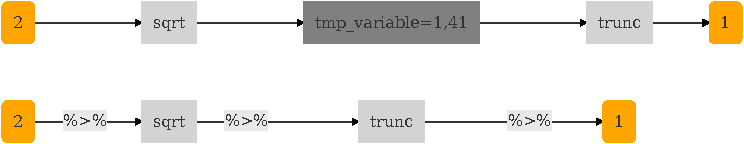
\includegraphics{tecnicas-cuantitativas_files/figure-latex/unnamed-chunk-26-1.pdf}
\caption{\label{fig:unnamed-chunk-26}Ejecución del código sin o con \texttt{\%\textgreater{}\%}. Sin \emph{pipes} los resultados intermedios tienen que guardarse en una variable en memoria.}
\end{figure}

Una operación compleja creada mediante el uso de \texttt{\%\textgreater{}\%} se puede usar en el lado derecho de una asignación \texttt{\textless{}-}, de modo que se guarda resultado de toda la operación de la derecha.

\begin{Shaded}
\begin{Highlighting}[]
\NormalTok{raiz_cuadrada_de_dos <-}\StringTok{ }\DecValTok{2} \OperatorTok
\StringTok{  }\KeywordTok{sqrt}\NormalTok{() }\OperatorTok
\StringTok{  }\KeywordTok{round}\NormalTok{(}\DataTypeTok{digits =} \DecValTok{2}\NormalTok{)}
\end{Highlighting}
\end{Shaded}

\hypertarget{ejercicios}{%
\section{Ejercicios}\label{ejercicios}}

Crea un \emph{script} para responder a cada pregunta. En las preguntas de la 4 a la 8 es posible que tengas que consultar la referencia de la librería \href{https://stringr.tidyverse.org/reference/index.html}{\texttt{stringr} (stringr.tidyverse.org/reference)} o a otras funciones de \texttt{R\ base}.

\begin{enumerate}
\def\labelenumi{\arabic{enumi}.}
\tightlist
\item
  Escribe un fragmento de código utilizando el operador \texttt{\%\textgreater{}\%} que haga lo siguiente:

  \begin{itemize}
  \tightlist
  \item
    tomar como entrada el número \texttt{1632}
  \item
    calcular el logaritmo en base 10
  \item
    redondear el número a la baja
  \item
    truncar la parte entera y
  \item
    verificar si se trata de un número entero.
  \end{itemize}
\item
  Escribe un fragmento de código utilizando el operador \texttt{\%\textgreater{}\%} que haga lo siguiente:

  \begin{itemize}
  \tightlist
  \item
    tomar como entrada el número \texttt{1632}
  \item
    calcular la raíz cuadrada,
  \item
    redondear al alza y quedarse con la parte entera, y
  \item
    verificar que se trata de un entero.
  \end{itemize}
\item
  Escribe un fragmento de código utilizando el operador \texttt{\%\textgreater{}\%} que haga lo siguiente:

  \begin{itemize}
  \tightlist
  \item
    tomar como entrada la cadena \texttt{1632}
  \item
    convertirla a número
  \item
    comprobar si el resultado es o no un número.
  \end{itemize}
\item
  Escribe un fragmento de código utilizando el operador \texttt{\%\textgreater{}\%} que haga lo siguiente:

  \begin{itemize}
  \tightlist
  \item
    tomar como entrada la cadena \texttt{"-16.32"}
  \item
    transformarla en un número
  \item
    calcular el valor absoluto y truncarlo
  \item
    comprobar si el resultado es o no un número.
  \end{itemize}
\item
  Escribe un fragmento de código utilizando el operador \texttt{\%\textgreater{}\%} y la librería and the \texttt{stringr} que haga lo siguiente:

  \begin{itemize}
  \tightlist
  \item
    tomar la cadena \texttt{"Siempre\ r\ que\ r"} como entrada
  \item
    transformar la cadena a mayúsculas.
  \end{itemize}
\item
  Escribe un fragmento de código utilizando el operador \texttt{\%\textgreater{}\%} y la librería and the \texttt{stringr} que haga lo siguiente:

  \begin{itemize}
  \tightlist
  \item
    tomar la cadena \texttt{"Siempre\ r\ que\ r"} como entrada
  \item
    truncarla para dejar solamente `Siempre R'.
  \end{itemize}
\end{enumerate}

\hypertarget{estaduxedstica-descriptiva}{%
\chapter{Estadística descriptiva}\label{estaduxedstica-descriptiva}}

La estadística descriptiva es una rama de la estadística cuyo objetivo es resumir, describir y presentar una serie de valores o un conjunto de datos. Estas estadísticas pueden ser realmente útiles al analizar largas series de datos en las que resulte difícil reconocer algún patrón. En éste capítulo utilizaremos una muestra de datos sobre salarios (en euros) de una \emph{población} de 100 trabajadores:

\emph{2186}, \emph{1218}, \emph{1682}, \emph{1816}, \emph{1702}, \emph{1447}, \emph{2256}, \emph{1453}, \emph{2509}, \emph{1469}, \emph{2152}, \emph{2643}, \emph{806}, \emph{1361}, \emph{1433}, \emph{1818}, \emph{1358}, \emph{172}, \emph{280}, \emph{2160}, \emph{1347}, \emph{609}, \emph{1414}, \emph{2107}, \emph{2448}, \emph{1285}, \emph{1371}, \emph{618}, \emph{1730}, \emph{1180}, \emph{1728}, \emph{1852}, \emph{2018}, \emph{1196}, \emph{1752}, \emph{642}, \emph{1108}, \emph{1074}, \emph{293}, \emph{1518}, \emph{1603}, \emph{1320}, \emph{1879}, \emph{1137}, \emph{816}, \emph{1716}, \emph{1094}, \emph{2222}, \emph{1284}, \emph{1828}, \emph{1661}, \emph{1108}, \emph{2288}, \emph{1821}, \emph{1545}, \emph{1638}, \emph{1840}, \emph{1545}, \emph{4}, \emph{1642}, \emph{1316}, \emph{1593}, \emph{1791}, \emph{2200}, \emph{1136}, \emph{2151}, \emph{1668}, \emph{2019}, \emph{1960}, \emph{1860}, \emph{978}, \emph{1455}, \emph{1812}, \emph{1023}, \emph{1229}, \emph{1790}, \emph{1884}, \emph{1732}, \emph{1057}, \emph{950}, \emph{2256}, \emph{1629}, \emph{1544}, \emph{1440}, \emph{903}, \emph{1806}, \emph{1391}, \emph{1409}, \emph{1967}, \emph{1911}, \emph{2196}, \emph{1262}, \emph{1825}, \emph{2196}, \emph{945}, \emph{1070}, \emph{934}, \emph{770}, \emph{1540} y \emph{1827}

De un primer vistazo es difícil (por no decir imposible) que podamos comprender los datos y tener una visión clara de los salarios de este grupo de personas. Las estadísticas descriptivas permiten resumir y así tener una mejor visión general de los datos. Por supuesto, al resumir los datos a través de una o varias medidas, inevitablemente se perderá parte de la información. Sin embargo, en muchos casos es mejor perder algo de información pero, a cambio, obtener una visión general. Podriamos decir que se trata de \emph{ganar perspectiva}.

La estadística descriptiva es a menudo el primer paso y una parte importante en cualquier análisis estadístico. Permite comprobar la calidad de los datos detectando posibles valores atípicos (\emph{outliers}), es decir, datos que parecen ser significativamente distintos del resto. También se puede utilizar estadística descriptiva para detectar errores de recopilación o codificación, determinar si están bien presentados, entre otras posibles aplicaciones.

Podemos distinguir dos típos básicos de estadísticos para describir un conjunto de datos: de centralidad y de dispersión. Habitualmente, ambos tipos de medidas se utilizan juntos para resumir los datos de la forma más concisa.

\hypertarget{tendencia-central}{%
\section{Tendencia central}\label{tendencia-central}}

Las medidas de tendencia central permiten ver ``dónde'' se ubican los datos, alrededor de qué valores. En otras palabras, las medidas de ubicación permiten comprender cuál es la tendencia central o la ``posición'' de los datos en su conjunto. Entre las estadísticas más habituales de este tipo podemos distinguir:

\begin{itemize}
\tightlist
\item
  Mínimo y máximo
\item
  Media
\item
  Mediana
\item
  Primer y tercer cuartil
\item
  Moda
\end{itemize}

\hypertarget{muxednimo-y-muxe1ximo}{%
\subsection{Mínimo y máximo}\label{muxednimo-y-muxe1ximo}}

Mínimo (\(min\)) y máximo (\(max\)) son simplemente los valores más bajo y más alto de la muestra. Dada una muestra de 6 de estos salarios:

\emph{2186}, \emph{1218}, \emph{1682}, \emph{1816}, \emph{1702} y \emph{1447}

El mínimo es 1217.7 euros y el máximo es 2185.5 euros. Estas dos estadísticas básicas dan una idea clara sobre el los extremos de la muestra y su cálculo con R es bastante sencillo:

\begin{Shaded}
\begin{Highlighting}[]
\KeywordTok{min}\NormalTok{(salarios_sel)}
\end{Highlighting}
\end{Shaded}

\begin{verbatim}
## [1] 1217.7
\end{verbatim}

\begin{Shaded}
\begin{Highlighting}[]
\KeywordTok{max}\NormalTok{(salarios_sel)}
\end{Highlighting}
\end{Shaded}

\begin{verbatim}
## [1] 2185.5
\end{verbatim}

\hypertarget{media}{%
\subsection{Media}\label{media}}

La media o promedio, es probablemente la estadística más habitual. Da una idea de cuál es el valor medio, es decir, el valor central de los datos o, en otras palabras, su centro de gravedad. La media se encuentra sumando todos los valores y dividiendo esta suma por el número de observaciones (\(n\)):

\[Media =\overline{x}=\frac{\text{suma de todos los valores}}{\text{número de valores}} = \frac{1}{n}\sum^{n}_{i=1}x_i\]
Dada nuestra muestra de 6 salarios presentada anteriormente, la media es:

\[\overline{x} = \frac{2186 + 1218 + 1682 + 1816 + 1702 + 1447}{6}= 1675,033\]

En conclusión, el tamaño medio de la nuestra muestra es 1675.03 euros (redondeado a 2 decimales). El cálculo con R también resulta bastante sencillo:

\begin{Shaded}
\begin{Highlighting}[]
\KeywordTok{mean}\NormalTok{(salarios_sel)}
\end{Highlighting}
\end{Shaded}

\begin{verbatim}
## [1] 1675.033
\end{verbatim}

\hypertarget{mediana}{%
\subsection{Mediana}\label{mediana}}

La mediana es otra medida de centralidad. La interpretación de la mediana es que hay tantas observaciones por debajo como por encima de la mediana. En otras palabras, el 50\% de las observaciones se encuentran por debajo de la mediana y el 50\% de las observaciones están por encima de la mediana.

La forma más fácil de calcular la mediana es primero ordenar los datos de menor a mayor (es decir, en orden ascendente) y luego tomar el punto medio como la mediana. A partir de los valores ordenados, para un número impar de observaciones, el punto medio es fácil de encontrar: es el valor con tantas observaciones abajo como arriba. Aún a partir de los valores ordenados, para un número par de observaciones, el punto medio está exactamente entre los dos valores medios. Formalmente, después de ordenar, la mediana es:

\begin{itemize}
\tightlist
\item
  si \(n\) (número de observaciones) es impar: \[mediana(x) = x_{\frac{n + 1}{2}}\]
\item
  si \(n\) es par: \[mediana(x) = \frac{1}{2}\big(x_{\frac{n}{2}} + x_{\frac{n}{2} + 1} \big)\]
\end{itemize}

donde el subíndice de \(x\) denota la numeración de los datos ordenados. El cálculo en R es de nuevo bastante sencillo:

\begin{Shaded}
\begin{Highlighting}[]
\KeywordTok{median}\NormalTok{(salarios_sel)}
\end{Highlighting}
\end{Shaded}

\begin{verbatim}
## [1] 1691.85
\end{verbatim}

\hypertarget{primer-y-tercer-cuartil}{%
\subsection{Primer y tercer cuartil}\label{primer-y-tercer-cuartil}}

El primer y tercer cuartil son similares a la mediana en el sentido de que también dividen las observaciones en dos partes, solo que estas partes no son iguales. Recordad que la mediana divide los datos en dos partes iguales (con el 50\% de las observaciones por debajo y el 50\% por encima de la mediana). El primer cuartil divide las observaciones de modo que haya un 25\% de las observaciones \emph{debajo de} este punto y un 75\% \textbf{por encima} del primer cuartil. El tercer cuartil se calcula del mismo modo pero representa el valor con el 75\% de las observaciones por debajo y el 25\% de las observaciones por encima. Existen varios métodos para calcular el primer y tercer cuartil, pero por ejemplo se puede calcular siguiendo los siguientes pasos:

\begin{enumerate}
\def\labelenumi{\arabic{enumi}.}
\tightlist
\item
  Ordenar los datos en orden ascendente
\item
  Calcular \(0.25\cdot n\) y \(0.75\cdot n\) (es decir, 0.25 y 0.75 veces el número de observaciones)
\item
  Redondear estos dos números al siguiente número entero \texttt{ceil}
\end{enumerate}

Los pasos son los mismos para un número par e impar de observaciones. A continuación se muestra un ejemplo para el cálculo de estos valores sobre los salarios de nueve trabajadores:

\begin{Shaded}
\begin{Highlighting}[]
\KeywordTok{quantile}\NormalTok{(salarios_sel)}
\end{Highlighting}
\end{Shaded}

\begin{verbatim}
##       0%      25%      50%      75%     100% 
## 1217.700 1505.575 1691.850 1787.825 2185.500
\end{verbatim}

Dado que obtenemos un vector de resultados, podemos seleccionar por posición para obtener el que necesitemos en cada caso.

\hypertarget{moda}{%
\subsection{Moda}\label{moda}}

La moda de una serie es el valor que aparece con mayor frecuencia. En otras palabras, es el valor que tiene el mayor número de ocurrencias. Dados los siguientes salarios:

\emph{1700}, \emph{1680}, \emph{1710}, \emph{1700}, \emph{1820}, \emph{1650}, \emph{1700}, \emph{1890} y \emph{1670}

La moda es 1700 porque es el valor más común con 3 apariciones. Todos los demás valores aparecen solo una vez. En conclusión, la mayoría de los trabajadores de esta muestra perciben exactamente 1700 euros al mes.

Hay que tener en cuenta que es posible que una serie no tenga moda (p.~Ej., \emph{4}, \emph{7}, \emph{2} y \emph{10}) o más de una moda (p.~Ej., \emph{4}, \emph{2}, \emph{2}, \emph{8}, \emph{11} y \emph{11}). Los datos con dos modas a menudo se denominan bimodales y los datos con más de dos modos a menudo se denominan multimodales, a diferencia de las series con una moda, que se denominan unimodales.

A diferencia de las anteriores estadísticas (mínimo, máximo, media, mediana, primer y tercer cuartil) que solo se pueden calcular para variables cuantitativas, \textbf{la moda se puede calcular para variables cuantitativas y cualitativas}. Atendiendo al tipo de empleo que desarrollan los 9 trabajadores presentados anteriormente:

\emph{ingeniero}, \emph{ingeniero}, \emph{ingeniero}, \emph{ingeniero}, \emph{asistente}, \emph{asistente}, \emph{asistente}, \emph{ingeniero} y \emph{camarero}

La moda es ``ingeniero'', por lo que la mayoría de los trabajadores de esta muestra son de uso ingenieros.

\hypertarget{dispersiuxf3n}{%
\section{Dispersión}\label{dispersiuxf3n}}

\hypertarget{rango}{%
\subsection{Rango}\label{rango}}

El rango es la diferencia entre el máximo y el mínimo:

\[rango = max - min\]

Dada nuestra muestra de salarios:

\emph{2186}, \emph{1218}, \emph{1682}, \emph{1816}, \emph{1702} y \emph{1447}

El rango es 2185.5 \(-\) 1217.7 \(=\) 967.8 euros. El rango es muy sencillo de calcular y en algunos casos puede dar una buena idea de lo que podemos esperar de un conjunto de datos. En R se puede utilizar la función \texttt{range}

\begin{Shaded}
\begin{Highlighting}[]
\KeywordTok{range}\NormalTok{(salarios_sel)}
\end{Highlighting}
\end{Shaded}

\begin{verbatim}
## [1] 1217.7 2185.5
\end{verbatim}

No obstante, esta métrica no da ninguna información de la distribución interna del resto de medidas.

\hypertarget{desviaciuxf3n-estuxe1ndard}{%
\subsection{Desviación estándard}\label{desviaciuxf3n-estuxe1ndard}}

La desviación estándar es la medida de dispersión más común en estadística. Si tenemos que presentar una estadística que resuma la distribución de los datos, suele ser la desviación estándar. Como sugiere su nombre, la desviación estándar indica cuál es la desviación \emph{normal} de los datos. De hecho, calcula la desviación promedio de la \textbf{media}. Cuanto mayor sea la desviación estándar, más dispersos estarán los datos. Por el contrario, cuanto menor es la desviación estándar, más se centran los datos alrededor de la media.

Existen dos fórmulas para calcular la desviación estándard en función de si nos enfrentamos a una muestra o a una población. Una población incluye a todos los miembros de un grupo específico, mientras que una muestra contiene algunas observaciones extraídas de la población, es decir, una parte o un subconjunto de la población. Por ejemplo, la población puede ser ``\textbf{todas} personas que viven en España'' y la muestra puede ser ``\textbf{algunas} personas que viven en España''.

La desviación estándar para una población, a partir de ahora \(\sigma\), es:

\[\sigma = \sqrt{\frac{1}{n}\sum^n_{i = 1}(x_i - \mu)^2}\]
Como se puede ver en la fórmula, la desviación estándar es en realidad la desviación promedio de los datos de su media \(\mu\). Hay calcular primero el cuadrado de la diferencia entre las observaciones y la media para evitar que las diferencias negativas se compensen con diferencias positivas.

Por ejemplo, imagine una población de solo 3 trabajadores:

\emph{770}, \emph{1540} y \emph{1827}

La media es 1379 (redondeado a 1 decimal). La desviación estándar es entonces:

\[\sigma = \sqrt{\frac{1}{3}\big[(770.4 - 1379)^2 + (1540 - 1379)^2 + (1827 - 1379)^2 \big]}\]
\[\sigma = 546,2\]

Por lo tanto, la desviación estándar para los salarios de estos trabajadores es de 546,2 euros. Esto significa que los salarios de los trabajadores de esta población se desvían de la media en 546,2 euros.

\ldots{}

\hypertarget{varianza}{%
\subsection{Varianza}\label{varianza}}

\hypertarget{coeficiente-de-variaciuxf3n}{%
\subsection{Coeficiente de variación}\label{coeficiente-de-variaciuxf3n}}

\hypertarget{correlaciuxf3n}{%
\section{Correlación}\label{correlaciuxf3n}}

Las correlaciones entre variables juegan un papel importante en un \textbf{análisis descriptivo}. Una correlación mide la \textbf{relación entre dos variables}, es decir, cómo están vinculadas entre sí. En este sentido, una correlación permite saber si dos variables evolucionan en la misma dirección, en sentido contrario y si son independientes.

En este capítulo, se muestra cómo calcular \textbf{coeficientes de correlación}, cómo realizar \textbf{pruebas de correlación} y cómo \textbf{visualizar} correlaciones entre variables usando R.

La correlación generalmente se calcula en dos variables \emph{cuantitativas}, pero también se puede calcular en dos variables \emph{cualitativas ordinales} (ver prueba de independencia de chi-cuadrado).

\hypertarget{datos}{%
\subsection{Datos}\label{datos}}

Usaremos el conjunto de datos \texttt{mtcars}. Este conjunto de datos viene cargado por defecto en R, de modo que se utiliza en numerosas demostraciones.

\begin{Shaded}
\begin{Highlighting}[]
\CommentTok{# mostrar las primeras cinco filas}
\KeywordTok{head}\NormalTok{(mtcars, }\DecValTok{5}\NormalTok{)}
\end{Highlighting}
\end{Shaded}

\begin{verbatim}
##                    mpg cyl disp  hp drat    wt  qsec vs am gear carb
## Mazda RX4         21.0   6  160 110 3.90 2.620 16.46  0  1    4    4
## Mazda RX4 Wag     21.0   6  160 110 3.90 2.875 17.02  0  1    4    4
## Datsun 710        22.8   4  108  93 3.85 2.320 18.61  1  1    4    1
## Hornet 4 Drive    21.4   6  258 110 3.08 3.215 19.44  1  0    3    1
## Hornet Sportabout 18.7   8  360 175 3.15 3.440 17.02  0  0    3    2
\end{verbatim}

Las variables \texttt{vs} y\texttt{am} son variables categóricas, por lo que se eliminan para este artículo:

\begin{Shaded}
\begin{Highlighting}[]
\CommentTok{# Eliminar las variables vs y am}
\KeywordTok{library}\NormalTok{(tidyverse)}
\NormalTok{dat <-}\StringTok{ }\NormalTok{mtcars }\OperatorTok
\KeywordTok{select}\NormalTok{(}\OperatorTok{-}\NormalTok{vs, }\OperatorTok{-}\NormalTok{am)}

\CommentTok{# mostrar las primeras cinco filas}
\KeywordTok{head}\NormalTok{(dat, }\DecValTok{5}\NormalTok{)}
\end{Highlighting}
\end{Shaded}

\begin{verbatim}
##                    mpg cyl disp  hp drat    wt  qsec gear carb
## Mazda RX4         21.0   6  160 110 3.90 2.620 16.46    4    4
## Mazda RX4 Wag     21.0   6  160 110 3.90 2.875 17.02    4    4
## Datsun 710        22.8   4  108  93 3.85 2.320 18.61    4    1
## Hornet 4 Drive    21.4   6  258 110 3.08 3.215 19.44    3    1
## Hornet Sportabout 18.7   8  360 175 3.15 3.440 17.02    3    2
\end{verbatim}

\hypertarget{coeficiente-de-correlaciuxf3n}{%
\subsection{Coeficiente de correlación}\label{coeficiente-de-correlaciuxf3n}}

La correlación entre 2 variables se calcula con la función \texttt{cor()}. Supón que queremos calcular la correlación entre caballos de potencia (\texttt{hp}) y millas por galón (\texttt{mpg}):

\begin{Shaded}
\begin{Highlighting}[]
\CommentTok{# Correlación de Pearson entre 2 variables }
\KeywordTok{cor}\NormalTok{(dat}\OperatorTok{$}\NormalTok{hp, dat}\OperatorTok{$}\NormalTok{mpg)}
\end{Highlighting}
\end{Shaded}

\begin{verbatim}
## [1] -0.7761684
\end{verbatim}

Hay que fijarse en que la correlación entre las variables \emph{X} e \emph{Y} es igual a la correlación entre las variables \emph{Y} y \emph{X}, por lo que el orden de las variables en la función \texttt{cor()} no importa.

La función \texttt{cor()} calcula por defecto la correlación de Pearson, por lo que si se quiere calcular la correlación por otro método, se puede agregar el argumento \texttt{method\ ="\ spearman\ "} a la función \texttt{cor()}:

\begin{Shaded}
\begin{Highlighting}[]
\CommentTok{# Correlación de Sperman entre 2 variables }
\KeywordTok{cor}\NormalTok{(dat}\OperatorTok{$}\NormalTok{hp, dat}\OperatorTok{$}\NormalTok{mpg,}
    \DataTypeTok{method =} \StringTok{"spearman"}\NormalTok{)}
\end{Highlighting}
\end{Shaded}

\begin{verbatim}
## [1] -0.8946646
\end{verbatim}

Hay varios métodos de correlación (se puede consultar la ayuda de la la función para saber más \texttt{?cor}):

\begin{itemize}
\tightlist
\item
  \textbf{Pearson} se usa a menudo para variables \emph{cuantitativas continuas} que tienen una relación lineal.
\item
  \textbf{Spearman} (es similar a Pearson pero se basa en los valores ordenados para cada variable en lugar de en los datos brutos) se usa a menudo para evaluar relaciones que involucran variables cualitativas ordinales en las que la relación sea parcialmente lineal.
\item
  \textbf{Kendall} se calcula a partir del número de pares concordantes y discordantes, se utiliza a menudo para variables ordinales cualitativas.
\end{itemize}

La función \texttt{cor\ ()} también permite calcular correlaciones para varios pares de variables a la vez:

\begin{Shaded}
\begin{Highlighting}[]
\CommentTok{# Correlaciones entre todas las variables}
\KeywordTok{round}\NormalTok{(}\KeywordTok{cor}\NormalTok{(dat),}
      \DataTypeTok{digits =} \DecValTok{2} \CommentTok{# redondeo a dos decimales}
\NormalTok{      ) }
\end{Highlighting}
\end{Shaded}

\begin{verbatim}
##        mpg   cyl  disp    hp  drat    wt  qsec  gear  carb
## mpg   1.00 -0.85 -0.85 -0.78  0.68 -0.87  0.42  0.48 -0.55
## cyl  -0.85  1.00  0.90  0.83 -0.70  0.78 -0.59 -0.49  0.53
## disp -0.85  0.90  1.00  0.79 -0.71  0.89 -0.43 -0.56  0.39
## hp   -0.78  0.83  0.79  1.00 -0.45  0.66 -0.71 -0.13  0.75
## drat  0.68 -0.70 -0.71 -0.45  1.00 -0.71  0.09  0.70 -0.09
## wt   -0.87  0.78  0.89  0.66 -0.71  1.00 -0.17 -0.58  0.43
## qsec  0.42 -0.59 -0.43 -0.71  0.09 -0.17  1.00 -0.21 -0.66
## gear  0.48 -0.49 -0.56 -0.13  0.70 -0.58 -0.21  1.00  0.27
## carb -0.55  0.53  0.39  0.75 -0.09  0.43 -0.66  0.27  1.00
\end{verbatim}

La correlación varía de \textbf{-1 a 1}, de modo que el signo nos indica la dirección de la relación (aumentan a la vez o son opuestas) y el valor nos indica la fuerza de la relación (más fuerte cuanto más alejado de 0).

Una \textbf{correlación negativa} implica que las dos variables consideradas varían en \textbf{direcciones opuestas}, es decir, si una variable aumenta la otra disminuye y viceversa. Por otro lado, una \textbf{correlación positiva} implica que las dos variables consideradas varían en la \textbf{misma dirección}, es decir, si una variable aumenta, la otra aumenta y si una disminuye, la otra también disminuye.

En cuanto a la fuerza de la relación: cuanto \textbf{más extremo} es el coeficiente de correlación (cuanto más cerca de -1 o 1), \textbf{más fuerte es la relación}. Esto también significa que una \textbf{correlación cercana a 0} indica que las dos variables son \textbf{independientes}, es decir, a medida que una variable aumenta, no hay tendencia en la otra variable a disminuir o aumentar.

Por ejemplo, la correlación de Pearson entre caballos de potencia (\texttt{hp}) y millas por galón (\texttt{mpg}) encontrada es -0.78, lo que significa que las 2 variables varían en dirección opuesta. Esto tiene sentido, los automoviles con más caballos de potencia suelen a consumir más combustible (hacen menos millas con el mismo combustible que los automóviles más potentes). Por el contrario, de la matriz de correlación vemos que la correlación entre millas por galón (\texttt{mpg}) y el tiempo para conducir un cuarto de milla (\texttt{qsec}) es 0.42, lo que significa que los automóviles rápidos (con un menor \texttt{qsec}) tienden a tener un peor rendimiento por galón (bajo \texttt{mpg}). De nuevo, esto tiene sentido, ya que los coches rápidos tienden a consumir más combustible.

\hypertarget{test-de-correlaciuxf3n}{%
\subsection{Test de correlación}\label{test-de-correlaciuxf3n}}

\begin{quote}
Volver una vez leída la sección sobre test de hipótesis.
\end{quote}

Hay que tener en cuenta que el valor \emph{p} se basa en el coeficiente de correlación y en el tamaño de la muestra. Cuanto mayor sea el tamaño de la muestra y más extrema será la correlación (más cercana a -1 o 1). Con un tamaño de muestra pequeño, es posible obtener una correlación \emph{relativamente} grande en la muestra (según el coeficiente de correlación), pero aún así encontrar una correlación no significativamente diferente de 0 en la población (según la prueba de correlación). Por este motivo, se recomienda realizar siempre un test de correlación antes de interpretar un coeficiente de correlación para evitar conclusiones erróneas.

A diferencia de una matriz de correlación que indica los coeficientes de correlación entre algunos pares de variables en la muestra, se utiliza un test de correlación para probar si la correlación (\(\rho\)) entre dos variables es significativamente diferente de 0 o no en la \emph{población}.

En realidad, un coeficiente de correlación diferente de 0 en la muestra no significa que la correlación sea \textbf{significativamente} diferente de 0 en la población. Esto debe probarse con un \textbf{test de hipótesis}.

Las hipótesis (nula y alternativa) para el test de correlación son las siguientes:

\begin{itemize}
\tightlist
\item
  \(H_0\): \(\rho = 0\) (si no existe una relación lineal entre las dos variables)
\item
  \(H_1\): \(\rho\ne 0\) (si existe una relación lineal entre las dos variables)
\end{itemize}

A través de esta prueba de correlación, lo que realmente estamos probando es si:

\begin{itemize}
\tightlist
\item
  La muestra contiene evidencia suficiente para rechazar la hipótesis nula y concluir que el coeficiente de correlación no es igual a 0, por lo que la relación existe en la población.
\item
  La muestra no contiene suficiente evidencia de que el coeficiente de correlación no sea igual a 0, por lo que en este caso no rechazamos la hipótesis nula de no-relación entre las variables de la población.
\end{itemize}

Supongamos que queremos probar si el ratio del eje trasero (\texttt{drat}) está correlacionado con el tiempo necesario para conducir 1/4 de milla (\texttt{qsec}):

\begin{Shaded}
\begin{Highlighting}[]
\CommentTok{# Test de correlación de Pearson}
\NormalTok{test <-}\StringTok{ }\KeywordTok{cor.test}\NormalTok{(dat}\OperatorTok{$}\NormalTok{drat, dat}\OperatorTok{$}\NormalTok{qsec)}
\NormalTok{test}
\end{Highlighting}
\end{Shaded}

\begin{verbatim}
## 
##  Pearson's product-moment correlation
## 
## data:  dat$drat and dat$qsec
## t = 0.50164, df = 30, p-value = 0.6196
## alternative hypothesis: true correlation is not equal to 0
## 95 percent confidence interval:
##  -0.265947  0.426340
## sample estimates:
##        cor 
## 0.09120476
\end{verbatim}

El \emph{p}-valor de la prueba de correlación entre estas 2 variables es 0.62. Al nivel de significancia del 5\%, no se rechaza la hipótesis nula de no correlación. Por lo tanto, concluimos que no rechazamos la hipótesis de que no existe una relación lineal entre las 2 variables. \footnote{Es importante recordar que probamos una relación \emph{lineal} entre las dos variables ya que usamos la correlación de Pearson. Puede darse el caso de que exista una relación entre las dos variables en la población, pero esta relación puede no ser lineal.}

Esta prueba demuestra que incluso si el coeficiente de correlación es diferente de 0 (la correlación es 0.09 en la muestra), en realidad no es significativamente diferente de 0 en la población.

\hypertarget{visualizando-correlaciones}{%
\subsection{Visualizando correlaciones}\label{visualizando-correlaciones}}

Una buena forma de visualizar una correlación entre 2 variables es mediante un diagrama de dispersión. Por ejemplo:

\begin{Shaded}
\begin{Highlighting}[]
\CommentTok{# Diagrama de dispersión con R base}
\KeywordTok{plot}\NormalTok{(dat}\OperatorTok{$}\NormalTok{hp, dat}\OperatorTok{$}\NormalTok{mpg)}
\end{Highlighting}
\end{Shaded}

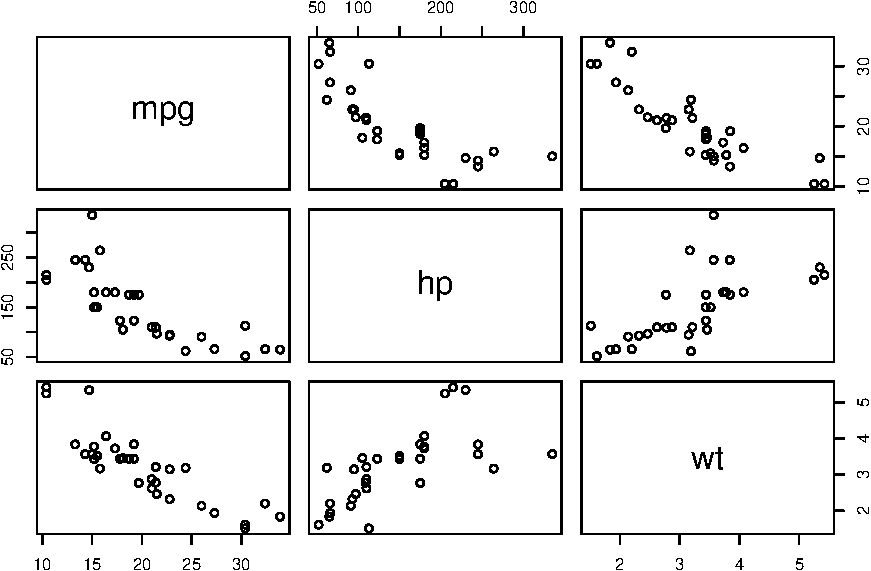
\includegraphics{tecnicas-cuantitativas_files/figure-latex/unnamed-chunk-45-1.pdf}

Para visualizar la relación entre más de 2 variablesse puede usar la función \texttt{pair\ ()}. En este caso limitamos el ejemplo a tres variables:

\begin{Shaded}
\begin{Highlighting}[]
\CommentTok{# Multiples diagramas de dispersión}
\KeywordTok{pairs}\NormalTok{(dat[, }\KeywordTok{c}\NormalTok{(}\DecValTok{1}\NormalTok{, }\DecValTok{4}\NormalTok{, }\DecValTok{6}\NormalTok{)])}
\end{Highlighting}
\end{Shaded}

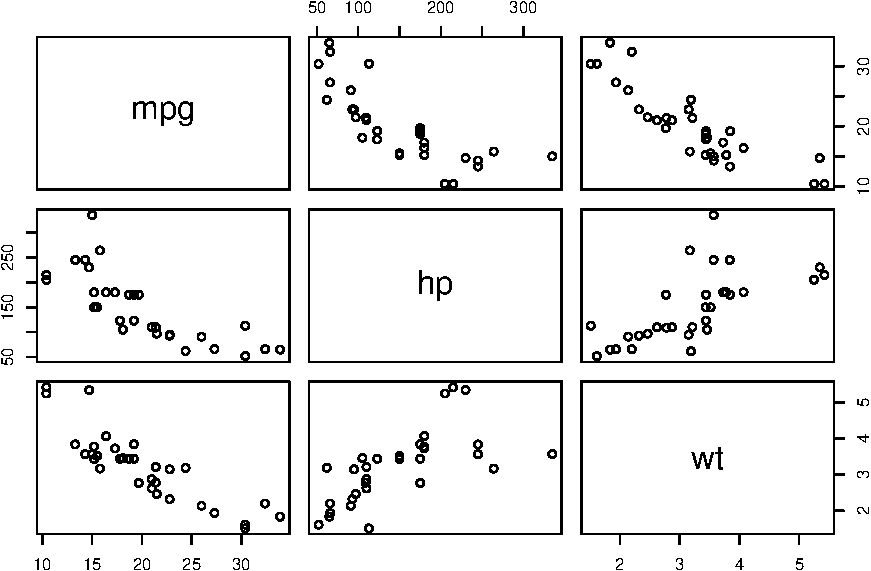
\includegraphics{tecnicas-cuantitativas_files/figure-latex/unnamed-chunk-46-1.pdf}

Por otra parte, existen numerosas librerías de R que permiten generar este tipo de gráficos con distintas opciones. Por ejemplo con \texttt{ggplot2}:

\begin{Shaded}
\begin{Highlighting}[]
\CommentTok{# Diagrama de dispersión con ggplot2}
\KeywordTok{library}\NormalTok{(ggplot2)}

\KeywordTok{ggplot}\NormalTok{(dat) }\OperatorTok{+}
\StringTok{ }\KeywordTok{aes}\NormalTok{(}\DataTypeTok{x =}\NormalTok{ hp, }\DataTypeTok{y =}\NormalTok{ mpg) }\OperatorTok{+}
\StringTok{ }\KeywordTok{geom_point}\NormalTok{(}\DataTypeTok{colour =} \StringTok{"#0c4c8a"}\NormalTok{) }\OperatorTok{+}
\StringTok{ }\KeywordTok{theme_minimal}\NormalTok{()}
\end{Highlighting}
\end{Shaded}

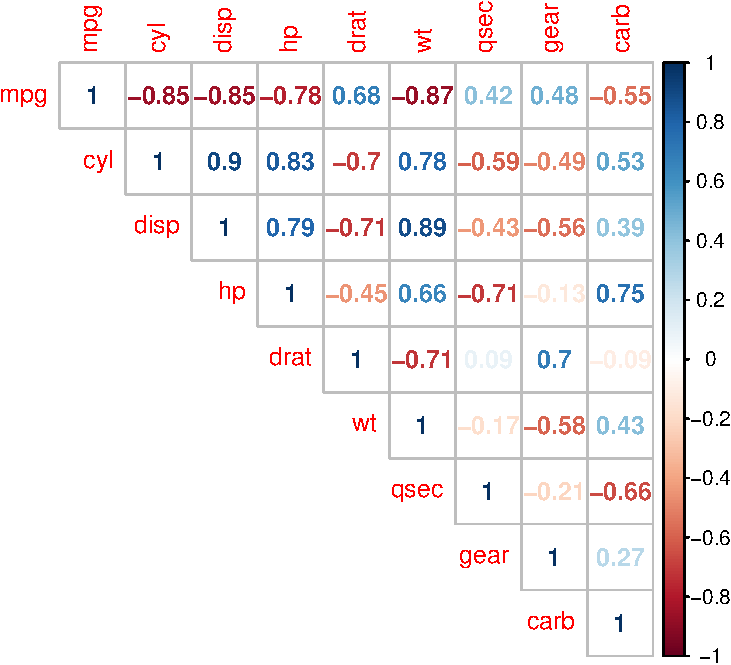
\includegraphics{tecnicas-cuantitativas_files/figure-latex/unnamed-chunk-47-1.pdf}

O representaciones más modernas como con la librería \texttt{corrplot}:

\begin{Shaded}
\begin{Highlighting}[]
\CommentTok{# improved correlation matrix}
\KeywordTok{library}\NormalTok{(corrplot)}

\KeywordTok{corrplot}\NormalTok{(}\KeywordTok{cor}\NormalTok{(dat),}
         \DataTypeTok{method =} \StringTok{"number"}\NormalTok{,}
         \DataTypeTok{type =} \StringTok{"upper"} \CommentTok{# show only upper side}
\NormalTok{         )}
\end{Highlighting}
\end{Shaded}

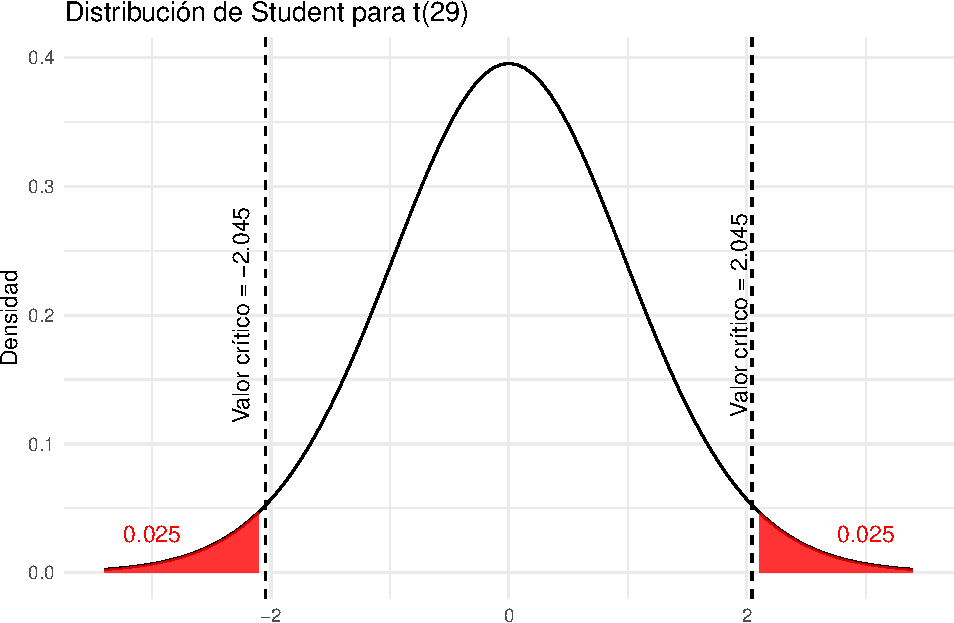
\includegraphics{tecnicas-cuantitativas_files/figure-latex/unnamed-chunk-48-1.pdf}

\hypertarget{ejercicios-1}{%
\section{Ejercicios}\label{ejercicios-1}}

\begin{enumerate}
\def\labelenumi{\arabic{enumi}.}
\tightlist
\item
  Estableced en clase un debate sobre variables de carácter territorial que consideréis que pueden estar correlacionadas y en qué medida.
\end{enumerate}

\hypertarget{estaduxedstica-inferencial}{%
\chapter{Estadística inferencial}\label{estaduxedstica-inferencial}}

La \textbf{estadísticas descriptiva} es la rama de las estadística que tiene como objetivo \textbf{describir y resumir un conjunto de datos} de la mejor manera posible, es decir, con la menor pérdida de información posible. Con la estadística descriptiva no hay incertidumbre, porque describimos solo el grupo de observaciones en las que decidimos trabajar y no se intenta generalizar las características observadas o estudiar un grupo más grande a partir de un conjunto de datos limitado.

Por otro lado, \textbf{La estadística inferencial} es la rama de la estadística que utiliza una muestra aleatoria de datos tomados de una población para hacer inferencias, es decir, \textbf{sacar conclusiones sobre la \emph{población} de interés}. En otras palabras, la información de la muestra se utiliza para hacer generalizaciones sobre el \emph{parámetro} de interés en la población.

Las dos herramientas más importantes utilizadas en estadística inferencial son los test de hipótesis y los intervalos de confianza.

\begin{quote}
Ver caso de bulos o noticias \emph{fake}
\end{quote}

La estadística inferencial proporciona las herramientas que necesitamos para responder a este tipo de preguntas, y dado que este tipo de preguntas y es una pieza fundamental de lo que podriamos denominar \textbf{lenguaje científico}. Sin embargo, la inferencia estadística se basa en la teoría de la probabilidad. Aquí no vamos a hablar de probabilidad pero, ya que la teoría de la probabilidad sustenta gran parte de las estadísticas, vale la pena cubrir algunos de los conceptos básicos.

\hypertarget{diferencia-entre-probabilidad-y-estaduxedstica}{%
\section{Diferencia entre probabilidad y estadística}\label{diferencia-entre-probabilidad-y-estaduxedstica}}

Probabilidad y estadística son dos disciplinas que están estrechamente relacionadas pero no son idénticas. La teoría de la probabilidad es \emph{``la doctrina de las posibilidades''}. Es una rama de las matemáticas que estiaud con qué frecuencia ocurrirán diferentes tipos de eventos. Por ejemplo, todas estas preguntas son cosas que puede responder usando la teoría de la probabilidad:

\begin{itemize}
\tightlist
\item
  ¿Cuáles son las posibilidades de que una moneda corriente salga cara 10 veces seguidas?
\item
  Si tiro dos dados de seis caras, ¿qué probabilidad hay de que saque dos seises?
\item
  ¿Qué posibilidades hay de que cinco cartas extraídas de una baraja perfectamente mezclada sean corazones?
\item
  ¿Cuáles son las posibilidades de que me toque la lotería?
\end{itemize}

Todas estas preguntas tienen algo en común. En cada caso, la \emph{``verdad''} se conoce de antemano, y cada pregunta se relaciona con ``qué tipo de eventos'' sucederán. En la primera pregunta, sabiendo que no se trata de una moneda trucada, hay un 50\% de posibilidades de que cualquier lanzamiento de moneda individual salga cara. En la segunda pregunta, sabemos que la posibilidad de sacar un 6 en un solo dado es de 1 entre 6. En la tercera pregunta, conocemos también el número de cartas y que han sido barajadas \emph{perfectamente}. En la cuarta pregunta, también se conocen las reglas específicas de cada juego (Euromillones, Primitiva, Loteria de Navidad, etc). El punto crítico es que las preguntas probabilísticas comienzan con un modelo conocido del mundo, y usamos ese modelo para hacer algunos cálculos. El modelo subyacente puede ser bastante simple. Por ejemplo, en el ejemplo del lanzamiento de una moneda, podemos escribir el modelo de esta manera:

\[
P(\mbox{caras}) = 0.5
\]
que se puede leer como ``la probabilidad de que salga cara es 0,5 sobre 1'' (las probabilidades son solo números que van del 0 al 1). Utilizamos este modelo pero, no se sabe exactamente lo que va a pasar. Todo es posible. Tal vez salgan diez caras, como dice la pregunta, pero tal vez consiga tres caras. Dicho de otro modo, en la teoría de la probabilidad, el modelo es conocido, pero los datos no.

En cambio, las preguntas estadísticas funcionan al revés. En estadística, no conocemos la ``verdad'' pero tenemos algunos datos, y es a partir de los datos que queremos aprender la ``verdad''. Las preguntas estadísticas tienden a parecerse más a estas:

\begin{itemize}
\tightlist
\item
  Si alguien lanza una moneda 10 veces y obtiene 10 caras, ¿me están haciendo trampas?
\item
  Si cinco cartas de la parte superior de la baraja son todos corazones, ¿qué probabilidad hay de que la baraja se haya barajado?
\item
  Si un político gana \emph{n} veces seguidas a la lotería, ¿qué probabilidades hay de que nos ensté engañando?
\end{itemize}

Esta vez, lo único que tenemos son datos. Se sabe lo que ha sucedido y se infiere si todo ha sucedido de un modo \emph{normal} o si hay alguna regla que no se ha respetado. Los datos que tenemos se ven así:

\begin{verbatim}
Cara Cara Cara Cara Cara Cara Cara Cara Cara Cara
\end{verbatim}

y lo que tratamos de averiguar es si debemos confiar en que esto sea ``verdad''. Si la moneda es una moneda común, entonces el modelo que debo adoptar es uno que diga que la probabilidad de que salga cara es 0.5; es decir, \(P(\mbox{caras}) = 0.5\). Si la moneda está trucada, entonces debería concluir que la probabilidad de que salga cara es \emph{no} 0.5, que escribiríamos como \(P(\mbox{caras})\neq0.5\). En otras palabras, el problema de la inferencia estadística es averiguar cuál de estos dos modelos de la realidad es el correcto. Así pues, la pregunta estadística no es la misma que la pregunta de probabilidad, pero están profundamente conectadas entre sí. Debido a esto, una buena introducción a la teoría estadística comenzará con una discusión sobre qué es la probabilidad y cómo funciona.

\hypertarget{probabilidad-frecuentista-vs-bayesiana}{%
\section{Probabilidad frecuentista vs Bayesiana}\label{probabilidad-frecuentista-vs-bayesiana}}

\hypertarget{enfoque-frecuentista}{%
\subsection{Enfoque frecuentista}\label{enfoque-frecuentista}}

El enfoque predominante para el estudio de la probabilidad en estadística, se conoce como \textbf{\emph{punto de vista frecuentista}}, y define la probabilidad como una \textbf{\emph{frecuencia a largo plazo}}. Lanzando una moneda que tiene \(P(caras) = 0.5\) podría suceder lo siguiente:

\begin{verbatim}
Cruz,Cara,Cara,Cara,Cara,Cruz,Cruz,Cara,Cara,Cara,Cara,Cruz,Cara,Cara,Cruz,Cruz,Cruz,Cruz,Cruz,Cara
\end{verbatim}

En este caso, 11 de estas 20 monedas (55\%) salieron cara. Ahora supongamos que he estado llevando un recuento continuo del número de caras (que llamaré \(N_{caras}\)) que he visto, en los primeros \(N\) volteos, y calculo la proporción de caras \(N_{caras}/N\) cada vez. Esto es lo que obtendría (¡literalmente lancé monedas para producir esto!):

\begin{tabular}{r|r|r}
\hline
Lanzamientos & Caras & Proporción\\
\hline
1 & 0 & 0.00\\
\hline
2 & 1 & 0.50\\
\hline
3 & 2 & 0.67\\
\hline
4 & 3 & 0.75\\
\hline
5 & 4 & 0.80\\
\hline
6 & 4 & 0.67\\
\hline
7 & 4 & 0.57\\
\hline
8 & 5 & 0.63\\
\hline
9 & 6 & 0.67\\
\hline
10 & 7 & 0.70\\
\hline
11 & 8 & 0.73\\
\hline
12 & 8 & 0.67\\
\hline
13 & 9 & 0.69\\
\hline
14 & 10 & 0.71\\
\hline
15 & 10 & 0.67\\
\hline
16 & 10 & 0.63\\
\hline
17 & 10 & 0.59\\
\hline
18 & 10 & 0.56\\
\hline
19 & 10 & 0.53\\
\hline
20 & 11 & 0.55\\
\hline
\end{tabular}

Al comienzo de la secuencia, la \emph{proporción} de caras fluctúa mucho, comenzando en .00 y subiendo hasta .80. Después de un cierto número de lanzamientos, da la impresión de que se la proporción disminuye un poco, y que cada vez más valores se acercan bastante a la respuesta que sabemo que es la ``correcta'' (.50). Esta es la definición \textbf{frecuentista} de probabilidad.

\begin{quote}
Lanza una moneda común una y otra vez, y a medida que \(N\) crece (se acerca al infinito, denotado \(N\rightarrow\infty\)), la proporción de caras se acercará al 50\%.
\end{quote}

Simulando con un ordenador es posible lanzar una moneda virtual 1000 veces para ver lo que sucede con la proporción \(N_{caras}/N\) a medida que aumenta \(N\). Los resultados se muestran en la Figura \ref{fig:frequentistprobability}. La \emph{proporción de caras observadas} finalmente deja de fluctuar y se estabiliza; cuando lo hace, el número en el que finalmente se asienta es la verdadera probabilidad de que salga cara.

\begin{figure}
\centering
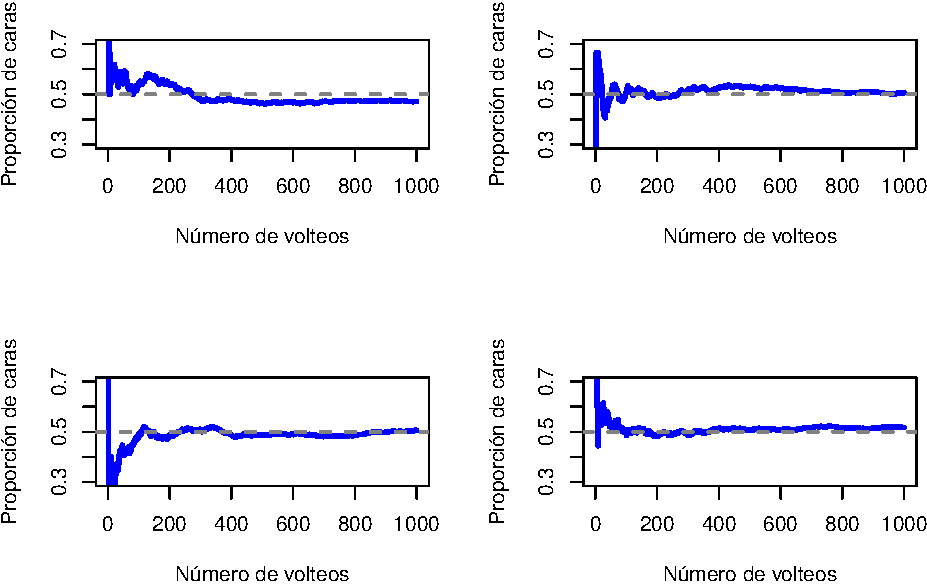
\includegraphics{tecnicas-cuantitativas_files/figure-latex/frequentistprobability-1.pdf}
\caption{\label{fig:frequentistprobability}Una ilustración de cómo funciona la probabilidad frecuentista. Si lanzamos una moneda una y otra vez, la proporción de caras que ha visto finalmente se estabiliza y converge a la probabilidad real de 0.5. Cada panel muestra cuatro experimentos simulados diferentes: en cada caso, simulamos que lanzamos una moneda 1000 veces y seguimos la pista de la proporción de lanzamientos que fueron caras a medida que avanzamos. Aunque ninguna de estas secuencias en realidad terminó con un valor exacto de .5, si hubiéramos extendido el experimento para un número infinito de lanzamientos de monedas, lo hubieran hecho.}
\end{figure}

La definición frecuentista de probabilidad resulta bastante interesante puesto que:
1. Es objetiva. La probabilidad de un evento está \emph{necesariamente} basada en el la realidad. Los enunciados de probabilidad pueden tener sentido si se refieren a (una secuencia de) eventos que ocurren en el universo físico.
2. Es inequívoca. Dos personas cualesquiera que observen el desarrollo de la misma secuencia de eventos, tratando de calcular la probabilidad de un evento, inevitablemente deben llegar a la misma respuesta.

Sin embargo, también hay que tener ciertas precauciones ya que:
1. Las secuencias infinitas no existen en el mundo físico. Por ejemplo, si se toma una moneda y se comienza a lanzar al suelo infinitas veces, cada vez que aterriza, impacta contra el suelo. Cada impacto desgasta un poco la moneda; eventualmente, la moneda quedará modificada y ya no volverá a ser la misma.
2. La definición frecuentista tiene un alcance limitado. Por ejemplo, si un meteorólogo aparece en la televisión y dice: ``la probabilidad de que llueva en Adelaida el 2 de noviembre de 2022 es del 60\%'', no está claro cómo definir esto en términos frecuentistas. Solo hay una ciudad de Adelaide, y solo habrà un 2 de noviembre de 2022. No hay una secuencia infinita de eventos aquí, solo una vez. La probabilidad frecuentista no contempla hacer enunciados de probabilidad sobre un solo evento. Desde la perspectiva frecuentista, mañana lloverá o no; no hay ``probabilidad'' que se adhiera a un solo evento no repetible.

\hypertarget{enfoque-bayesiano}{%
\subsection{Enfoque Bayesiano}\label{enfoque-bayesiano}}

El enfoque bayesiana de la probabilidad a menudo se denomina visión subjetivista, y es una visión minoritaria entre los estadísticos, pero que ha ido ganando terreno de manera constante durante las últimas décadas. La forma más común de pensar sobre la probabilidad subjetiva es definir la probabilidad de un evento como el grado de creencia que alguien inteligente y racional asigna a la probabilidad de ese evento. Según esto, las probabilidades no existen en el mundo, sino en los pensamientos y suposiciones de las personas. Sin embargo, para que este enfoque funcione, necesitamos alguna forma de operacionalizar ``grado de creencia''. Supongamos que creo que hay un 60\% de probabilidad de que llueva mañana. Si alguien me ofrece una apuesta: si mañana llueve, gano 5 euros, pero si no llueve, pierdo 5 euros. Claramente, desde mi perspectiva, esta es una apuesta bastante buena. Por otro lado, si creo que la probabilidad de lluvia es solo del 40\%, entonces es una mala apuesta. Por lo tanto, podemos operacionalizar la noción de una ``probabilidad subjetiva'' en términos de las apuestas que estoy dispuesto a aceptar.

¿Cuáles son las ventajas y desventajas del enfoque bayesiano? La principal ventaja es que te permite asignar probabilidades a cualquier evento. No es necesario que se limite a los eventos que se pueden repetir. La principal desventaja es que no podemos ser puramente objetivos: especificar una probabilidad requiere que especifiquemos una entidad que tenga el grado de creencia relevante. Esta entidad puede ser un humano, un extraterrestre, un robot o incluso un estadístico, pero tiene que haber un agente inteligente que crea en las cosas. Para mucha gente esto es incómodo: parece hacer que la probabilidad sea arbitraria. Si bien el enfoque bayesiano requiere que el agente en cuestión sea racional (es decir, obedezca las reglas de probabilidad), sí permite que todos tengan sus propias creencias; Puedo creer que la moneda es común y tú no tienes que hacerlo, aunque ambos seamos racionales. La visión frecuentista no permite que dos observadores atribuyan diferentes probabilidades al mismo evento: cuando eso sucede, al menos uno de ellos debe estar equivocado. La visión bayesiana no evita que esto ocurra. Dos observadores con conocimientos previos diferentes pueden tener legítimamente creencias diferentes sobre el mismo evento. En resumen, donde la visión frecuentista a veces se considera demasiado estrecha (prohíbe muchas cosas a las que queremos asignar probabilidades), la visión bayesiana a veces se piensa que es demasiado amplia (permite demasiadas diferencias entre observadores).

\hypertarget{introducciuxf3n-a-las-distribuciones-de-probabilidad}{%
\section{Introducción a las distribuciones de probabilidad}\label{introducciuxf3n-a-las-distribuciones-de-probabilidad}}

Una distribución de probabilidad es una función que describe la probabilidad de obtener los posibles valores que puede asumir una variable aleatoria. En otras palabras, los valores de la variable varían según la distribución de probabilidad subyacente.

Supongamos que seleccionamos una muestra aleatoria de personas y medimos la altura de los sujetos. A medida que vamos midiendo las alturas, podemos crear una distribución de alturas. Este tipo de distribución es útil cuando necesita saber qué resultados son más probables, la dispersión de los valores potenciales y la probabilidad de resultados diferentes. Por lo tanto se puede utilizar distribuciones de probabilidad para realizar inferencias.

\begin{quote}
Ejemplo a partir de la película ``El sargento de hierro'' de Clint Eastwood.
\end{quote}

Supongamos que el profesor solo tiene 5 jerseis (\(X_1\), \(X_2\), \(X_3\), \(X_4\) y \(X_5\). Cada prenda (es decir, cada \(X\)) sería un \textbf{\emph{evento elemental}}. La característica clave de los eventos elementales es que cada vez que hacemos una observación (por ejemplo, cada vez que me pongo un jersey), el resultado será uno y solo uno de estos eventos. De manera similar, el conjunto de todos los eventos posibles se denomina \textbf{\emph{espacio muestral}}.

Definido el espacio muestral, que se construye a partir de muchos posibles eventos elementales (jerseys), lo que queremos hacer es asignar una \textbf{\emph{probabilidad}} de uno de estos eventos elementales. Para un evento \(X\), la probabilidad de ese evento \(P(X)\) es un número que se encuentra entre 0 y 1. Cuanto mayor sea el valor de \(P(X)\), es más probable que ocurra el evento. Entonces, por ejemplo, si \(P(X)=0\), significa que el evento \(X\) es imposible (es decir, nunca uso ese jersey). Por otro lado, si \(P(X)=1\) significa que el evento \(X\) seguramente ocurrirá (es decir, siempre uso ese jersey). Todos los demas valores, entre 0 y 1, significarían que unas veces uso un jersey y otras veces otros. Por ejemplo, si \(P(X)=0.5\) significa que uso ese jersey la mitad del tiempo.

Las probabilidades de los todos los eventos elementales deben sumar 1. Esto se conoce como la \textbf{\emph{ley de la probabilidad total}}. Si se satisfacen estos requisitos, entonces lo que tenemos es una \textbf{\emph{distribución de probabilidad}}. Por ejemplo, este es un ejemplo de distribución de probabilidad

\begin{tabular}{l|l|l|l|l|l}
\hline
Jersey & Azul & Gris & Naranja & Amarillo & Marrón\\
\hline
Etiqueta & \$X\_1\$ & \$X\_2\$ & \$X\_3\$ & \$X\_4\$ & \$X\_5\$\\
\hline
Probabildad & \$P(X\_1) = .5\$ & \$P(X\_2) = .3\$ & \$P(X\_3) = .1\$ & \$P(X\_4) = 0\$ & \$P(X\_5) = .1\$\\
\hline
\end{tabular}

Cada uno de los eventos tiene una probabilidad que se encuentra entre 0 y 1, y si sumamos la probabilidad de todos los eventos, suman 1. Impresionante. Incluso podemos dibujar un bonito gráfico de barras para visualizar esta distribución, como se muestra en la Figura \ref{pantsprob}.

\begin{figure}
\centering
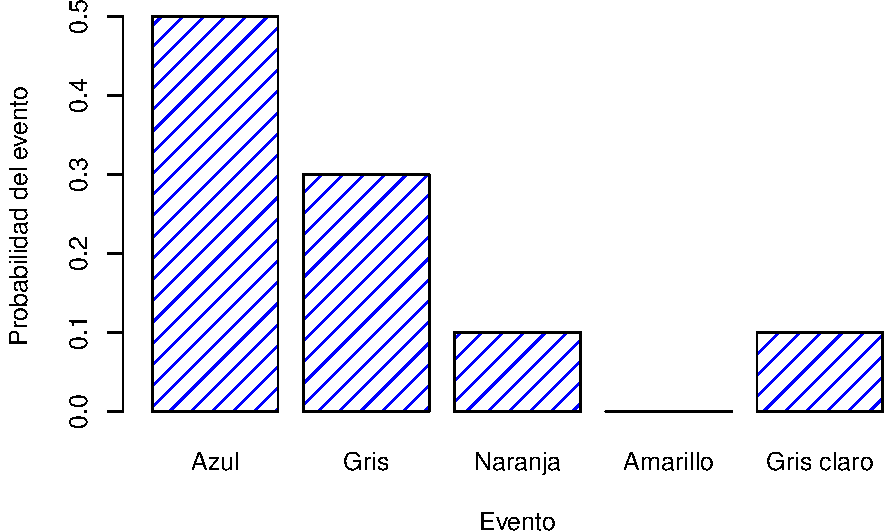
\includegraphics{tecnicas-cuantitativas_files/figure-latex/pantsprob-1.pdf}
\caption{\label{fig:pantsprob}Representación visual de la distribución de probabilidad de jerseys del profesor. Hay cinco eventos elementales, correspondientes a los cinco jerseys. Cada evento tiene alguna probabilidad de ocurrir: esta probabilidad es un número entre 0 y 1. La suma de estas probabilidades es 1.}
\end{figure}

Cabe ser señalado es que la teoría de la probabilidad permite hablar de eventos elementales y también de \textbf{\emph{eventos no elementales}}. En el ejemplo de los jerseys, es perfectamente legítimo referirse a la probabilidad de que vista un color claro. En términos matemáticos, definimos el evento ``jersey de color claro'' \(E\) para que corresponda al conjunto de eventos elementales \((X_1, X_2, X_3)\). Si ocurre alguno de estos eventos elementales, también se dice que ha ocurrido \(E\). Habiendo decidido escribir la definición de \(E\) de esta manera, es bastante sencillo establecer cuál es la probabilidad \(P(E)\): simplemente sumamos todo. En este caso particular
\[
P(E) = P(X_1) + P(X_2) + P(X_3)
\]
y, dado que las probabilidades de los jerseys amarillo, naranja y gris claro, respectivamente, son .1, 0 y .1, la probabilidad de que use un jersey de color claro es igual a .2.

A partir de estos principios tan simples es posible construir algunas herramientas matemáticas extremadamente poderosas. En la Tabla \ref{tab:probrules} aparecen algunas de las otras reglas que satisfacen las probabilidades.

\begin{table}

\caption{\label{tab:probrules}Algunas reglas básicas que deben cumplir las probabilidades.}
\centering
\begin{tabular}[t]{l|l|l|l}
\hline
Expresión & Notación & NANA & Formula\\
\hline
No \$A\$ & \$P(\textbackslash{}neg A)\$ & = & \$1-P(A)\$\\
\hline
\$A\$ o \$B\$ & \$P(A \textbackslash{}cup B)\$ & = & \$P(A) + P(B) - P(A \textbackslash{}cap B)\$\\
\hline
\$A\$ y \$B\$ & \$P(A \textbackslash{}cap B)\$ & = & \$P(A|B) P(B)\$\\
\hline
\end{tabular}
\end{table}

Las distribuciones de probabilidad varían enormemente. Sin embargo, no todas son igualmente importantes. Las más utilizadas serían: la distribución binomial, la distribución normal, la distribución \(t\), la distribución \(\ chi^2\) (``chi-cuadrado'') y la distribución distribución de \(F\). Aquí prestaremos especial atención a la binomial y a la normal.

\hypertarget{la-distribuciuxf3n-binomial}{%
\subsection{La distribución binomial}\label{la-distribuciuxf3n-binomial}}

La teoría de la probabilidad se originó en el intento de describir cómo funcionan los juegos de azar, por lo que parece apropiado que nuestra discusión sobre la \textbf{\emph{distribución binomial}} incluya una discusión sobre el lanzamiento de dados y monedas. Imaginemos un ``experimento'' simple: en un cubilete hay 20 dados idénticos de seis caras. En una cara de cada dado hay una imagen de un bufón (\emph{joker}) y las otras cinco caras están todas en blanco. Si lanzamos los 20 dados, ¿cuál es la probabilidad de que obtenga exactamente 4 \emph{jokers}? Suponiendo que los dados no estén trucados, sabemos que la probabilidad de que se obtenga un \emph{joker} es de 1 en 6; Para decir esto de otra manera, la probabilidad de \emph{joker} para un solo dado es aproximadamente \(.167\).

Si \(N\) es el número de tiradas de dados en nuestro experimento; que a menudo se denomina \textbf{\emph{parámetro de tamaño}} de nuestra distribución binomial. Mientras que \(\theta\) es la probabilidad de que un solo dado produzca un \emph{joker}, una cantidad que generalmente se llama \textbf{\emph{probabilidad de éxito}} del binomio. Finalmente, \(X\) serán resultados de nuestro experimento, es decir, el número de \emph{jokers} obtenido al tirar los dados. Dado que el valor real de \(X\) se debe al azar, nos referimos a él como \textbf{\emph{variable aleatoria}}. La cantidad que queremos calcular es la probabilidad de que \(X=4\) dado que sabemos que \(\theta=.167\) y \(N=20\). La ``forma'' general de lo que me interesa calcular podría escribirse como

\[
P(X \ | \ \theta, N)
\]
y estamos interesados en el caso especial donde \(X=4\), \(\theta=.167\) y \(N=20\). Si quiero decir que \(X\) se genera aleatoriamente a partir de una distribución binomial con los parámetros \(\theta\) y \(N\), la notación que usaría es la siguiente:
\[
X \sim \mbox{Binomial}(\theta, N)
\]
La distribución binomial tiene el aspecto que muestar en la Figura \ref{fig:binomial1} y traza las probabilidades binomiales para todos los valores posibles de \(X\). Si se lanzan los dados, desde \(X=0\) (sin \emph{jokers}) hasta \(X=20\) (todos los jokers). Esto es básicamente un gráfico de barras, y no es diferente del gráfico de ``probabilidad de jerseys''de la Figura \ref{fig:pantsprob}. En el eje horizontal tenemos todos los eventos posibles y en el eje vertical podemos leer la probabilidad de cada uno de esos eventos. Entonces, la probabilidad de sacar 4 \emph{jokers} de 20 veces es de aproximadamente 0.20. En otras palabras, esperaría que eso sucediera aproximadamente el 20\% de las veces que se lancen los dados.

\begin{figure}
\centering
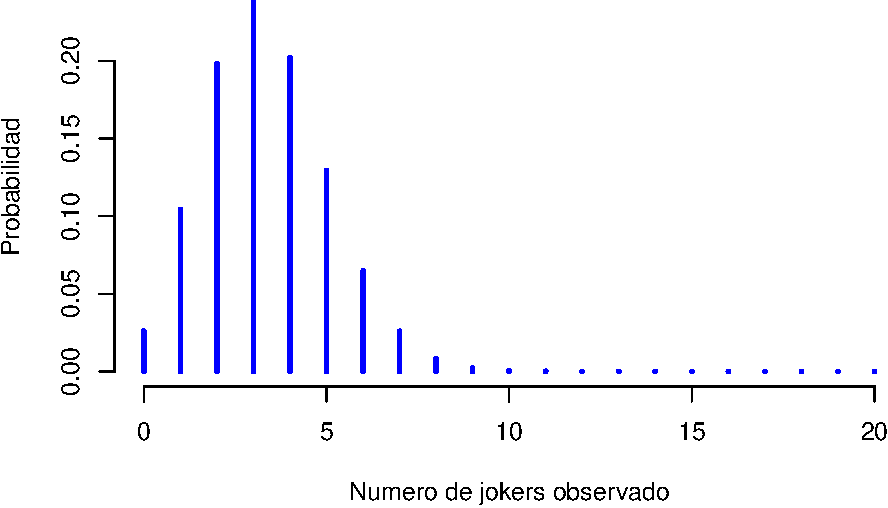
\includegraphics{tecnicas-cuantitativas_files/figure-latex/binomial1-1.pdf}
\caption{\label{fig:binomial1}La distribución binomial con parámetro de tamaño de \(N=20\) y una probabilidad de éxito subyacente de \(theta=1/6\). Cada barra vertical representa la probabilidad de un resultado específico (es decir, un valor posible de \(X\)). Debido a que esta es una distribución de probabilidad, cada una de las probabilidades debe ser un número entre 0 y 1, y las alturas de las barras también deben sumar 1.}
\end{figure}

Como se ha visto en la tabla \ref{tab:probability-functions}, R tiene una función llamada \texttt{dbinom\ ()} que calcula probabilidades binomiales. Los principales argumentos de la función son:

\begin{itemize}
\tightlist
\item
  \texttt{x}. Éste es un número o vector, que especifica los resultados cuya probabilidad se está tratando de calcular.
\item
  \texttt{size}. Este es un número que le dice a R el tamaño del experimento.
\item
  \texttt{prob}. Ésta es la \emph{probabilidad de éxito} de cualquier ensayo del experimento.
\end{itemize}

Entonces, para calcular la probabilidad de obtener \texttt{x\ =\ 4} \emph{jokers}, a partir de un experimento de \texttt{size\ =\ 20} ensayos, en el que la probabilidad de obtener un \emph{joker} en cualquier ensayo es \texttt{prob\ =\ 1/6}, el comando que usaríamos es:

\begin{Shaded}
\begin{Highlighting}[]
\KeywordTok{dbinom}\NormalTok{( }\DataTypeTok{x =} \DecValTok{4}\NormalTok{, }\DataTypeTok{size =} \DecValTok{20}\NormalTok{, }\DataTypeTok{prob =} \DecValTok{1}\OperatorTok{/}\DecValTok{6}\NormalTok{ )}
\end{Highlighting}
\end{Shaded}

\begin{verbatim}
## [1] 0.2022036
\end{verbatim}

Para ver cómo cambia la distribución binomial cuando modificamos los valores de \(\theta\) y \(N\), cambiemos los dados por monedas. De este modo, la probabilidad de éxito ahora es \(\theta=1/2\). Suponiendo que se lanzara la moneda \(N=20\) veces. Es decir que estamos cambiando la probabilidad de éxito, pero manteniendo el tamaño del experimento. Como muestra la Figura \ref{fig:binomial2a}, el efecto principal de esto es cambiar toda la distribución. ¿Y si lanzamos una moneda \(N=100\) veces? Bueno, en ese caso, se obtiene la distribución que aparece en la Figura \ref{fig:binomial2b}. La distribución se mantiene aproximadamente en el medio, pero hay un poco más de variabilidad en los posibles resultados.

\begin{figure}
\centering
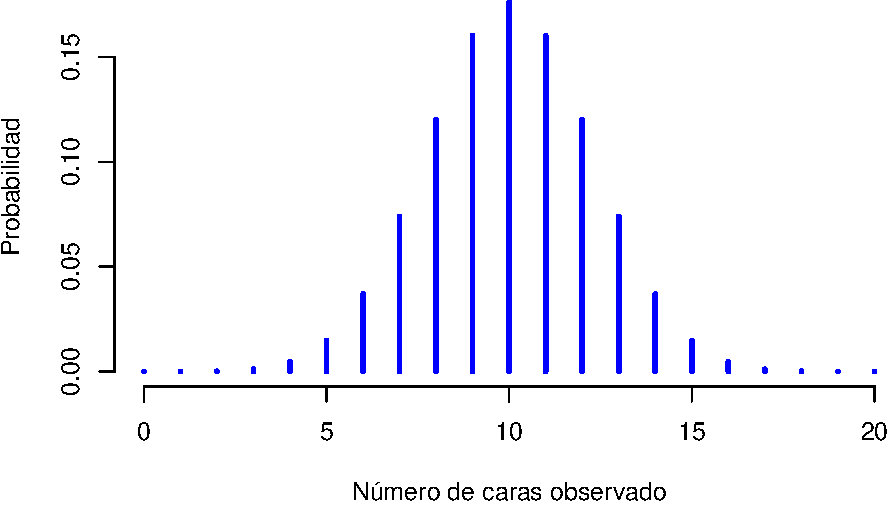
\includegraphics{tecnicas-cuantitativas_files/figure-latex/binomial2a-1.pdf}
\caption{\label{fig:binomial2a}Dos distribuciones binomiales, que involucran un escenario en el que estoy lanzando una moneda, por lo que la probabilidad de éxito subyacente es \(theta=1/2\). Aquí asumimos que estoy lanzando la moneda \(N=20\) veces.}
\end{figure}

\begin{figure}
\centering
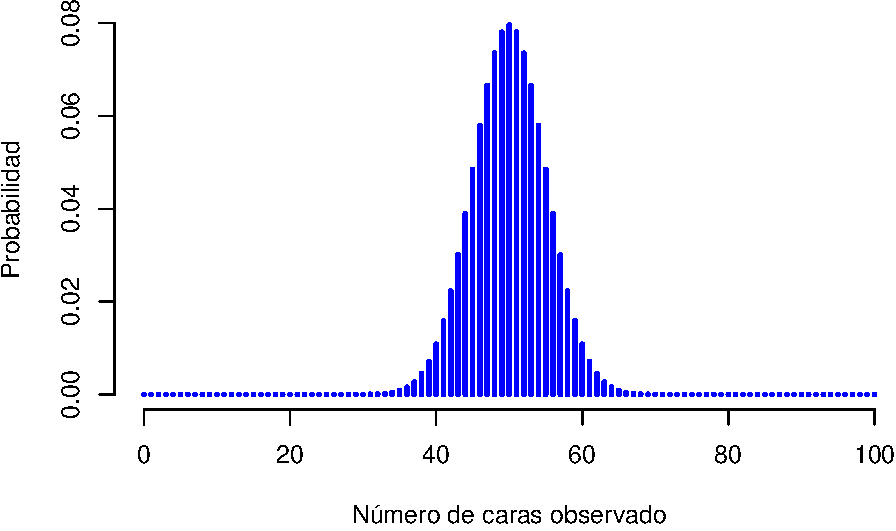
\includegraphics{tecnicas-cuantitativas_files/figure-latex/binomial2b-1.pdf}
\caption{\label{fig:binomial2b}Dos distribuciones binomiales, que involucran un escenario en el que se lanza una moneda, por lo que la probabilidad de éxito subyacente es \(theta=1/2\). Aquí asumimos que la moneda se lanza \(N=100\) veces.}
\end{figure}

La fórmula de la distribución binomial que calcula R es la siguiente:
\(P(X | \theta, N) = \displaystyle\frac{N!}{X! (N-X)!} \theta^X (1-\theta)^{N-X}\)

\hypertarget{la-distribuciuxf3n-normal}{%
\subsection{La distribución normal}\label{la-distribuciuxf3n-normal}}

La fórmula de la distribución normal que calcula R es la siguiente:
\(p(X | \mu, \sigma) = \displaystyle\frac{1}{\sqrt{2\pi}\sigma} \exp \left( -\frac{(X - \mu)^2}{2\sigma^2} \right)\)

\begin{figure}
\centering
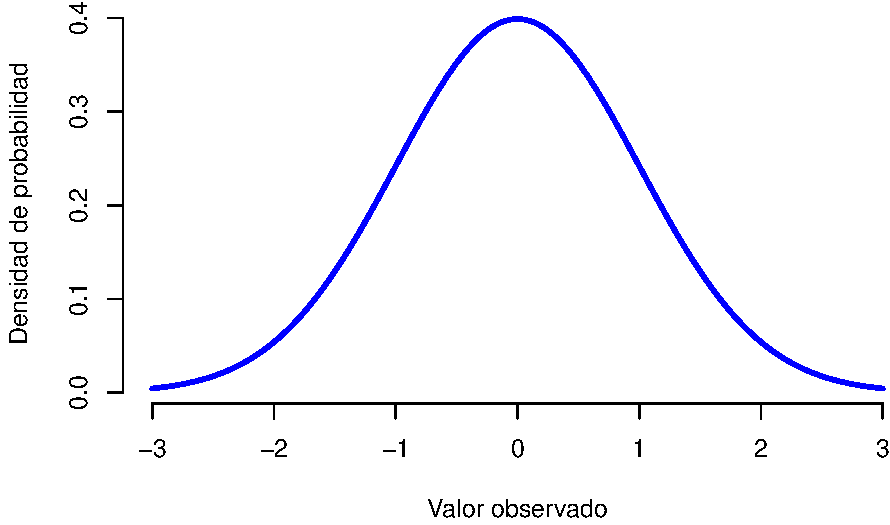
\includegraphics{tecnicas-cuantitativas_files/figure-latex/normdist-1.pdf}
\caption{\label{fig:normdist}\{La distribución normal con media \(mu=0\) y desviación estándar \(sigma = 1\). El eje \(x\) corresponde al valor de alguna variable, y el eje \(y\) nos dice algo sobre la probabilidad de que observemos ese valor. Sin embargo, observe que el eje \(y\) está etiquetado como ``Densidad de probabilidad'' y no como ``Probabilidad''. Existe una característica sutil y algo frustrante de las distribuciones continuas que hace que el eje \(y\) se comporte un poco extraño: la altura de la curva aquí no es en realidad la probabilidad de observar un valor particular de \(x\). Por otro lado, \emph{es} cierto que las alturas de la curva indican qué valores de \(x\) son más probables.}
\end{figure}

La \textbf{\emph{distribución normal}}, que también se conoce como ``de campana'' o una ``distribución gaussiana'' es la distribución más utilizada. Una distribución normal se describe usando dos parámetros, la media de la distribución \(\mu\) y la desviación estándar de la distribución \(\sigma\). La notación que a veces usamos para decir que una variable \(X\) se distribuye normalmente es la siguiente:

\[
X \sim \mbox{Normal}(\mu,\sigma)
\]

\hypertarget{funciones-de-r-para-distribuciones-de-probabilidad}{%
\subsection{Funciones de R para distribuciones de probabilidad}\label{funciones-de-r-para-distribuciones-de-probabilidad}}

R tiene varias funciones para trabajar con cada distribución de probabilidad. Hay un nombre de raíz, por ejemplo, el nombre de raíz para la distribución normal es \texttt{norm}. Esta raíz tiene como prefijo una de las letras:

\begin{itemize}
\tightlist
\item
  \texttt{p} para ``probabilidad'', la función de distribución acumulativa.
\item
  \texttt{q} para ``cuantil'', el inverso de la función de distribución acumulativa.
\item
  \texttt{d} para ``densidad'', la función de densidad.
\item
  \texttt{r} para ``aleatorio'', una variable aleatoria que tiene la distribución especificada.
\end{itemize}

Las cuatro versiones de la cada función requieren que especifiquen los argumentos \texttt{size} y\texttt{prob}. Sin embargo, difieren en términos de cuál es el otro argumento y cuál es el resultado:

\begin{itemize}
\tightlist
\item
  La forma \texttt{d} requiere un resultado particular\texttt{x}, y el devuelve la probabilidad de obtener exactamente ese resultado.
\item
  La forma \texttt{p} calcula la \textbf{\emph{probabilidad acumulada}}. Se le da un cuantil particular \texttt{q}, y se le dice la probabilidad de obtener un resultado \emph{menor o igual que} \texttt{q}.
\item
  La forma \texttt{q} calcula los \textbf{\emph{cuantiles}} de la distribución. Se especifica un valor de probabilidad \texttt{p} y devuelve el percentil correspondiente. Es decir, el valor de la variable para el que existe una probabilidad \texttt{p} de obtener un resultado menor que ese valor.
\item
  La forma \texttt{r} es un \textbf{\emph{generador de números aleatorios}}: específicamente, genera \texttt{n} resultados aleatorios de la distribución.
\end{itemize}

Para la distribución normal, estas funciones son \texttt{pnorm}, \texttt{qnorm}, \texttt{dnorm} y \texttt{rnorm}, mientras que para la distribución binomial, estas funciones son \texttt{pbinom}, \texttt{qbinom}, \texttt{dbinom} y \texttt{rbinom}.

Para una distribución continua (como la normal), las funciones más útiles para resolver problemas que involucran cálculos de probabilidad son las funciones \texttt{p} y \texttt{q}, porque la densidad por la función \texttt{d} solo se puede usar para calcular probabilidades a través de integrales.

Para una distribución discreta (como la binomial), la función \texttt{d} calcula la densidad, Que en este caso es una probabilidad

\(f(x) = P(X = x)\)

y por lo tanto es útil para calcular probabilidades.

R tiene funciones para manejar muchas distribuciones de probabilidad. La siguiente tabla proporciona los nombres de las funciones para cada distribución y un enlace a la documentación en línea que es la referencia autorizada sobre cómo se utilizan las funciones. Pero no lea la documentación en línea todavía. Primero, pruebe los ejemplos de las secciones que siguen a la tabla.

\begin{table}[!h]

\caption{(\#tab:table:probability-functions)Funciones para distribución de probabilidades in R.}
\centering
\fontsize{12}{14}\selectfont
\begin{tabular}[t]{>{\raggedright\arraybackslash}p{0.5in}>{\raggedright\arraybackslash}p{0.7in}>{\raggedright\arraybackslash}p{1in}>{\raggedright\arraybackslash}p{1.1in}>{\raggedright\arraybackslash}p{1in}}
\toprule
Distribution & p & q & d & r\\
\midrule
Beta & pbeta & qbeta & dbeta & rbeta\\
Binomial & pbinom & qbinom & dbinom & rbinom\\
Cauchy & pcauchy & qcauchy & dcauchy & rcauchy\\
Chi-Square & pchisq & qchisq & dchisq & rchisq\\
Exponential & pexp & qexp & dexp & rexp\\
F & pf & qf & df & rf\\
Gamma & pgamma & qgamma & dgamma & rgamma\\
Geometric & pgeom & qgeom & dgeom & rgeom\\
Hypergeometric & phyper & qhyper & dhyper & rhyper\\
Logistic & plogis & qlogis & dlogis & rlogis\\
Log Normal & plnorm & qlnorm & dlnorm & rlnorm\\
Negative Binomial & pnbinom & qnbinom & dnbinom & rnbinom\\
Normal & pnorm & qnorm & dnorm & rnorm\\
Poisson & ppois & qpois & dpois & rpois\\
Student t & pt & qt & dt & rt\\
Studentized Range & ptukey & qtukey & dtukey & rtukey\\
Uniform & punif & qunif & dunif & runif\\
Weibull & pweibull & qweibull & dweibull & rweibull\\
Wilcoxon Rank Sum Statistic & pwilcox & qwilcox & dwilcox & rwilcox\\
Wilcoxon Signed Rank Statistic & psignrank & qsignrank & dsignrank & rsignrank\\
\bottomrule
\end{tabular}
\end{table}

\hypertarget{ejemplos-con-la-distribuciuxf3n-binomial}{%
\subsection{Ejemplos con la distribución Binomial}\label{ejemplos-con-la-distribuciuxf3n-binomial}}

De nuevo, si lanzamos dados, y cada dado tiene una probabilidad de 1 en 6 de obtener \emph{jokers}, supongamos, que queremos saber la probabilidad de sacar 4 \emph{o menos} jockers. Podríamos usar la función \texttt{dbinom\ ()} para calcular la probabilidad exacta de obtener 0 \emph{jokers}, 1 \emph{joker}, 2 \emph{jokers}, 3 \emph{jokers} y 4 \emph{jokers} y luego sumarlas, pero hay una manera más rápida. En su lugar, se puede usar la función \texttt{pbinom\ ()}:

\begin{Shaded}
\begin{Highlighting}[]
\KeywordTok{pbinom}\NormalTok{(}\DataTypeTok{q=} \DecValTok{4}\NormalTok{, }\DataTypeTok{size =} \DecValTok{20}\NormalTok{, }\DataTypeTok{prob =} \DecValTok{1}\OperatorTok{/}\DecValTok{6}\NormalTok{)}
\end{Highlighting}
\end{Shaded}

\begin{verbatim}
## [1] 0.7687492
\end{verbatim}

En otras palabras, hay un 76,9\% de posibilidades de que saque 4 \emph{jokers} o menos. R dice que un valor de 4 es en realidad el percentil 76,9 de esta distribución binomial.

A continuación, consideremos la función \texttt{qbinom\ ()}. Digamos que queremos calcular el percentil 75 de la distribución binomial. Siguiendo con el ejemplo de los dados:

\begin{Shaded}
\begin{Highlighting}[]
\KeywordTok{qbinom}\NormalTok{( }\DataTypeTok{p =} \FloatTok{0.75}\NormalTok{, }\DataTypeTok{size =} \DecValTok{20}\NormalTok{, }\DataTypeTok{prob =} \DecValTok{1}\OperatorTok{/}\DecValTok{6}\NormalTok{)}
\end{Highlighting}
\end{Shaded}

\begin{verbatim}
## [1] 4
\end{verbatim}

Lo que la función \texttt{qbinom\ ()} parece estar diciendo es que el percentil 75 de la distribución binomial es 4, aunque según en la función \texttt{pbinom\ ()} se sabe que 4 es \emph{en realidad} el percentil 76,9. La rareza aquí proviene del hecho de que nuestra distribución binomial realmente no \emph{tiene} un percentil 75. Hay un 56,7\% de posibilidades de sacar 3 \emph{jokers} o menos (ver \texttt{pbinom\ (3,\ 20,\ 1/6)}) y un 76,9\% de posibilidades de sacar 4 calaveras o menos. Entonces, en cierto sentido el percentil 75 debería estar ``entre'' 3 y 4 \emph{jockers}. Pero aquí los decimales no tienen sentido. Este problema se puede manejar de diferentes maneras:

\begin{enumerate}
\def\labelenumi{\arabic{enumi}.}
\tightlist
\item
  Se puede informar un valor intermedio (o un valor \emph{interpolado}) como 3.9,
\item
  Se puede redondear a la baja (a 3) o hacia arriba (a 4).
\end{enumerate}

La función \texttt{qbinom\ ()} redondea hacia arriba si se solicita un percentil que en realidad no existe (como el 75 en este ejemplo), R encuentra el valor más pequeño para el cual el rango percentil es \emph{al menos} lo que se pidió. En este caso, dado que el percentil 75 ``verdadero'' se encuentra entre 3 y 4 \emph{jokers}, R redondea y devuelve un valor de 4. Esto solo es un problema para distribuciones discretas como la binomial.

Finalmente, tenemos el generador de números aleatorios (\texttt{rbinom\ ()}). Hay que especificar cuántas veces R debe ``simular'' el experimento usando el argumento \texttt{n}, y generará resultados aleatorios a partir de la distribución binomial. Entonces, por ejemplo, supongamos que se tuviera que repetir el experimento de lanzamiento de dados 100 veces. Podría hacer que R simule los resultados de estos experimentos usando el siguiente comando:

\begin{Shaded}
\begin{Highlighting}[]
\KeywordTok{rbinom}\NormalTok{( }\DataTypeTok{n =} \DecValTok{100}\NormalTok{, }\DataTypeTok{size =} \DecValTok{20}\NormalTok{, }\DataTypeTok{prob =} \DecValTok{1}\OperatorTok{/}\DecValTok{6}\NormalTok{ )}
\end{Highlighting}
\end{Shaded}

\begin{verbatim}
##   [1] 3 1 4 5 3 4 1 2 4 3 3 5 6 6 6 6 3 4 1 3 3 4 3 3 2 2 3 5 3 4 4 5 3 6 4 6 3
##  [38] 5 2 3 4 3 6 3 0 2 1 3 1 4 4 4 5 1 2 5 7 6 4 6 4 1 3 3 4 3 4 2 2 2 2 2 2 2
##  [75] 2 2 3 3 6 4 3 4 2 5 4 2 3 3 6 8 2 2 4 5 2 2 2 5 1 4
\end{verbatim}

Como puede ver, estos números son más o menos los que se puede ver en la Figura @ref(fig: binomial1). La mayoría de las veces se obtienen entre 1 y 5 \emph{jokers}.

\hypertarget{ejemplos-con-la-distribuciuxf3n-normal}{%
\subsection{Ejemplos con la distribución normal}\label{ejemplos-con-la-distribuciuxf3n-normal}}

Como ya se ha dicho, las funciones R para la distribución normal son \texttt{dnorm\ ()}, \texttt{pnorm\ ()}, \texttt{qnorm\ ()} y \texttt{rnorm\ ()}. Sin embargo, se comportan prácticamente de la misma manera que las funciones correspondientes para la distribución binomial, por lo que no hay mucho que deba saber. Únicamente, cabe mencionar, que los nombres de los argumentos para los parámetros son \texttt{mean} y\texttt{sd}.

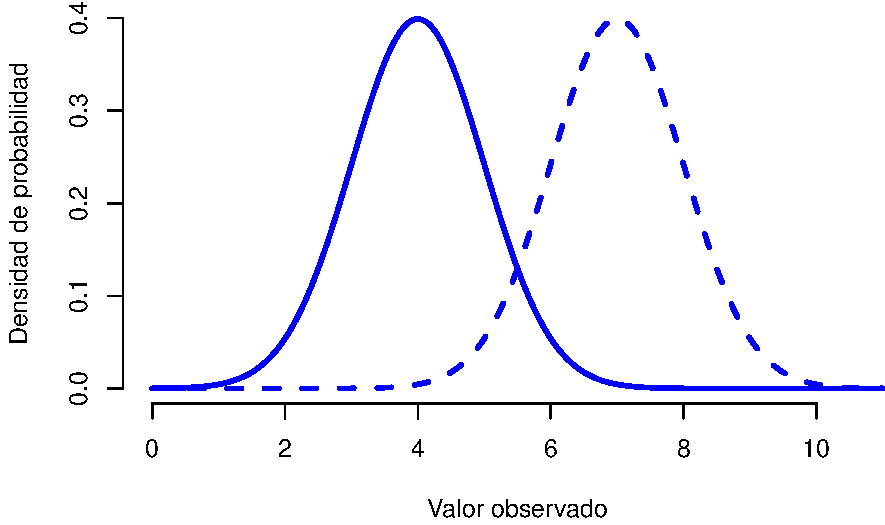
\includegraphics{tecnicas-cuantitativas_files/figure-latex/normmean-1.pdf}
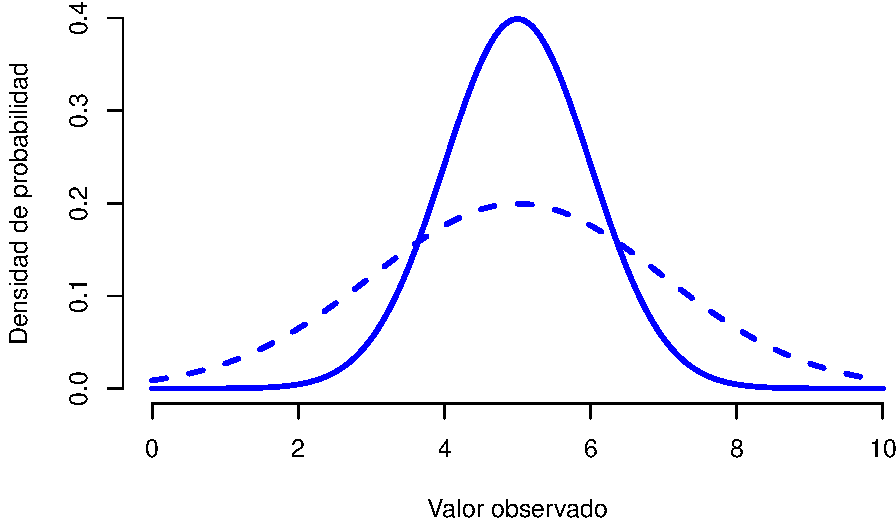
\includegraphics{tecnicas-cuantitativas_files/figure-latex/normsd-1.pdf}

En la Figura \ref{fig:normdist}, se traza una distribución normal con media \(\mu=0\) y desviación estándar \(\sigma=1\). En vez de un histograma, la imagen de la distribución normal en la Figura \ref{fig:normdist} muestra una curva suave. Esta no es una elección arbitraria: la distribución normal es continua, mientras que la binomial es discreta. Las escalas continuas no tienen esta restricción. Por ejemplo, la temperatura de un día de primavera podría ser de 23 grados, 24 grados, 23,9 grados o cualquier punto intermedio, ya que la temperatura es una variable continua, por lo que una distribución normal podría ser muy apropiada para describir las temperaturas de primavera.

\begin{quote}
Mencionar el caso de las escalas Likert
\end{quote}

La Figura \ref{fig:normmean} traza distribuciones normales que tienen diferentes medias, pero tienen la misma desviación estándar. Como era de esperar, todas estas distribuciones tienen el mismo ``ancho''. La única diferencia entre ellos es que se han desplazado hacia la izquierda o hacia la derecha. En todos los demás aspectos, son idénticos. Por el contrario, si aumentamos la desviación estándar mientras mantenemos la media constante, el pico de la distribución permanece en el mismo lugar, pero la distribución se ensancha, como puede ver en la Figura \ref{fig:normsd}. Sin embargo, cuando ampliamos la distribución, la altura del pico se reduce. Esto tiene que suceder: de la misma manera que las alturas de las barras que usamos para dibujar una distribución binomial discreta tienen que \emph{suma } 1, el área total \emph{bajo la curva} para la distribución normal debe ser igual a 1. No obstante, independientemente de cuál sea la media real y la desviación estándar, el 68,3\% del área se encuentra dentro de 1 desviación estándar de la media. Del mismo modo, el 95,4\% de la distribución se encuentra dentro de 2 desviaciones estándar de la media y el 99,7\% de la distribución está dentro de 3 desviaciones estándar. Esta idea se ilustra en la Figura \ref{fig:sdnorm}.

\begin{figure}
\centering
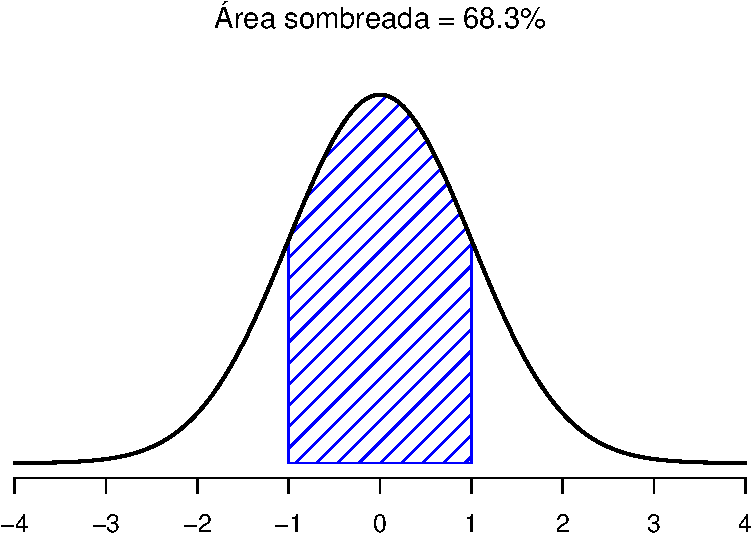
\includegraphics{tecnicas-cuantitativas_files/figure-latex/sdnorm1a-1.pdf}
\caption{\label{fig:sdnorm1a}El área debajo de la curva indica la probabilidad de que una observación se encuentre dentro de un rango particular. Las líneas continuas trazan distribuciones normales con media \(mu=0\) y desviación estándar \(sigma=1\). Las áreas sombreadas ilustran ``áreas bajo la curva'' para dos casos importantes. Aquí podemos ver que hay un 68,3\% de probabilidad de que una observación caiga dentro de una desviación estándar de la media.}
\end{figure}

\begin{figure}
\centering
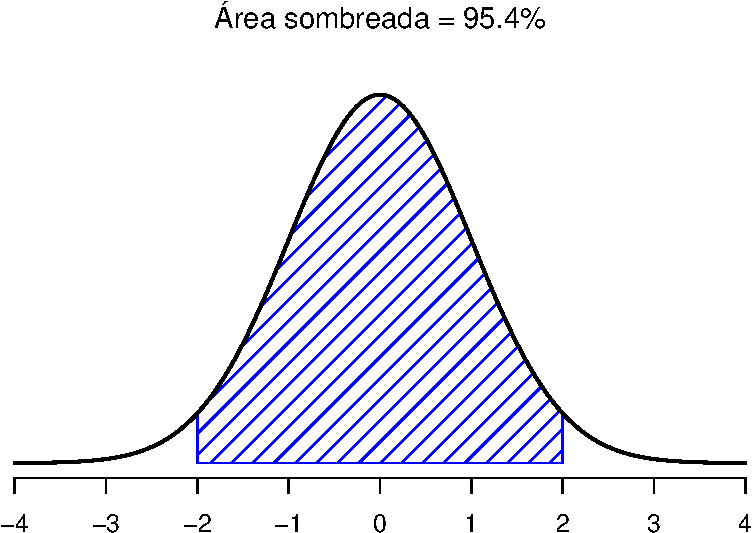
\includegraphics{tecnicas-cuantitativas_files/figure-latex/sdnorm1b-1.pdf}
\caption{\label{fig:sdnorm1b}El área debajo de la curva indica la probabilidad de que una observación se encuentre dentro de un rango particular. Las líneas continuas trazan distribuciones normales con media \(mu = 0\) y desviación estándar \(sigma = 1\). Las áreas sombreadas ilustran ``áreas bajo la curva'' para dos casos importantes. Aquí vemos que hay un 95,4\% de probabilidad de que una observación caiga dentro de dos desviaciones estándar de la media.}
\end{figure}

\begin{figure}
\centering
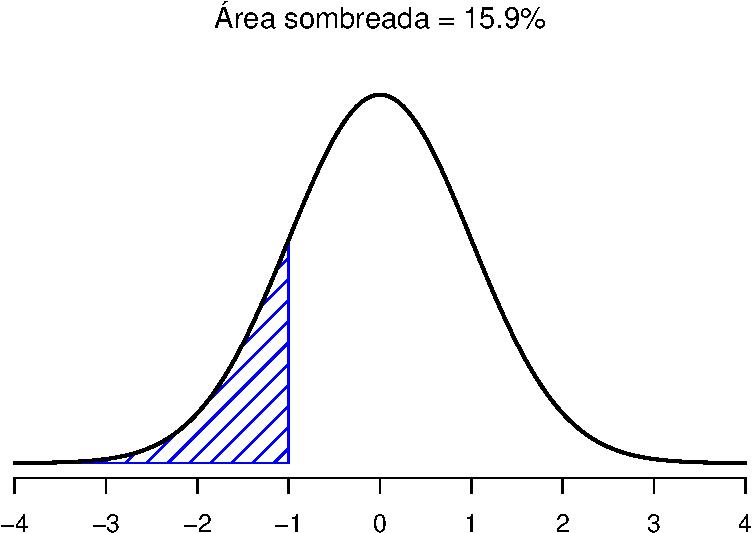
\includegraphics{tecnicas-cuantitativas_files/figure-latex/sdnorm2a-1.pdf}
\caption{\label{fig:sdnorm2a}Dos ejemplos más de la ``idea del área bajo la curva''. Hay un 15.9\% de probabilidad de que una observación esté una desviación estándar por debajo de la media o menor.}
\end{figure}

\begin{figure}
\centering
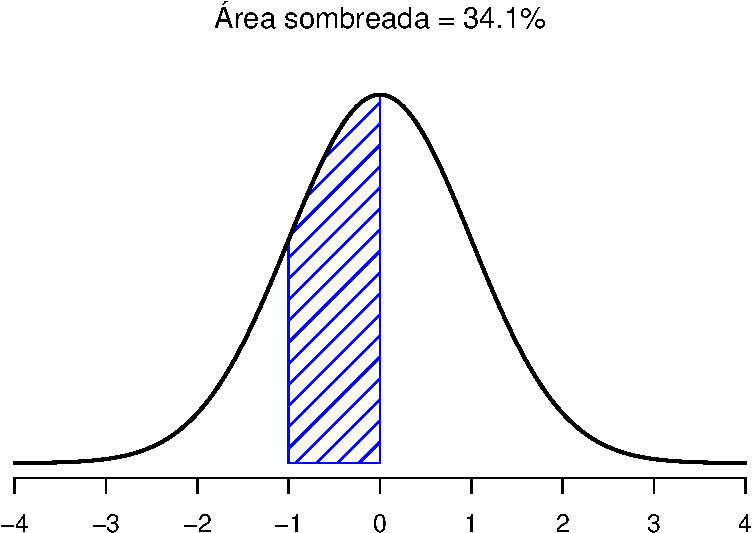
\includegraphics{tecnicas-cuantitativas_files/figure-latex/sdnorm2b-1.pdf}
\caption{\label{fig:sdnorm2b}Existe una probabilidad del 34,1\% de que la observación sea mayor que una desviación estándar por debajo de la media pero aún por debajo de la media. Si suma estos dos números, se obtiene \(15.9 + 34.1 = 50\). Para datos distribuidos normalmente, existe un 50\% de probabilidad de que una observación caiga por debajo de la media. Y, por supuesto, eso también implica que hay un 50\% de probabilidad de que esté por encima de la media.}
\end{figure}

\hypertarget{introduccion-a-los-test-de-hipuxf3tesis}{%
\section{Introduccion a los test de hipótesis}\label{introduccion-a-los-test-de-hipuxf3tesis}}

Primero cabe preguntarse por qué intentaríamos hacer inferencias sobre un parámetro de una población basadonos en una muestra, en lugar de simplemente recopilar datos para toda la población, calcular estadísticas que nos interesan y tomar decisiones basadas en eso. La principal razón por la que utilizamos una muestra en lugar de toda la población es porque recopilar datos sobre toda la población es más compicado o en ocasiones impracticable por varios motivos (complejidad, coste, limitación de tiempo, entre muchos otros motivos). \footnote{Por ejemplo, una investigación podría consistir en conocer si la población de la provincia de Tarragona está satisfecha con el nuevo plan de movilidad. Si pudiéramos preguntar a toda la población en un período de tiempo razonable, no haríamos ninguna estadística inferencial. No obstante, aún habria que decidir que preguntas se les hace para entender mejor el motivo de su grado de satisfacción, complicando y encareciendo aún más la encuesta.}

\begin{quote}
El objetivo general de una prueba de hipótesis es sacar conclusiones para confirmar o refutar una creencia sobre una población basándonos en un grupo más pequeño de observaciones.
\end{quote}

Las pruebas de hipótesis tienen muchas aplicaciones prácticas. Aquí ponemos algunos ejemplos:

\begin{enumerate}
\def\labelenumi{\arabic{enumi}.}
\tightlist
\item
  Una media: supongamos que a un político le gustaría le gustaría probar si el salario medio de los trabajadores españoles es diferente de 1200 euros.
\item
  Dos medias:

  \begin{itemize}
  \tightlist
  \item
    Muestras independientes: supongamos que a un profesor le gustaría probar la idoneidad de un nuevo método docente midiendo la nota media para los alumnos de un grupo de control y los del grupo en el que se ha introducido la novedad.
  \item
    Muestras pareadas o relacionadas: supongamos que el mismo profesor quisiera probar la idoneidad de este nuevo método de enseñanza pero lo hiciera midiendo los conocimientos de los alumnos antes y después de la explicación.
  \end{itemize}
\item
  Una proporción: supongamos que a un analísta político quisiera comprobar si la proporción de ciudadanos que van a votar por un candidato específico es inferior al 25\%.
\item
  Dos proporciones: supongamos que a un geógrafo le gustaría probar si la proporción de visitantes a una playa es diferente entre jóvenes y personas mayores.
\item
  Una variación: supongamos que un ingeniero quisiera probar si una batería tiene una variabilidad en el timpo de carga menor que la indicada en la descripción técnica.
\item
  Dos variaciones: supongamos que, en una fábrica, dos líneas de producción funcionan independientemente una de la otra. El gerente querría probar si los costes del mantenimiento semanal de estas dos cadenas de producción tienen la misma variación.
\end{enumerate}

Por supuesto, hay muchísimas más aplicaciones potenciales y muchas preguntas de investigación pueden responderse gracias a una prueba de hipótesis.

Por lo general, \textbf{las pruebas de hipótesis se utilizan para responder preguntas de investigación en análisis confirmatorios}. Los análisis confirmatorios se refieren a análisis estadísticos donde las hipótesis --- deducidas de la teoría --- se definen de antemano (preferiblemente antes de la recopilación de datos). En este enfoque, la investigadora tiene una idea específica sobre las variables en consideración y está tratando de ver si su idea, especificada como hipótesis, está respaldada por datos.

Podemos utilizar al menos tres métodos diferentes para realizar una prueba de hipótesis comparando:

\begin{enumerate}
\def\labelenumi{\arabic{enumi}.}
\tightlist
\item
  la estadística de prueba con el \textbf{valor crítico}.
\item
  el \textbf{\emph{p}-valor} con el nivel de significancia \(\alpha\).
\item
  el parámetro objetivo con el \textbf{intervalo de confianza}.
\end{enumerate}

Estos enfoques puede diferir en algunos aspectos pero tienen muchos puntos en común. El uso de uno u otro método es a menudo una cuestión de elección personal o de contexto.

Para los tres métodos, explicaré los pasos necesarios para realizar una prueba de hipótesis desde un punto de vista general y los ilustraré con la siguiente situación: \footnote{Puede ver más o menos pasos en otros artículos o libros de texto, dependiendo de si estos pasos son detallados o concisos. Sin embargo, la prueba de hipótesis debe seguir el mismo proceso independientemente del número de pasos}.

\begin{quote}
Supongamos que un político quisiera comprobar si el salario medio de los trabajadores españoles es diferente de 1.200 euros.
\end{quote}

En la mayoría de las pruebas de hipótesis, la prueba que vamos a utilizar como ejemplo a continuación requiere algunas condiciones. En esta sección asumimos que se cumplen todos los supuestos pero más adelante hablaremos de esto.

\hypertarget{comparando-la-estaduxedstica-de-prueba-con-el-valor-cruxedtico.}{%
\subsection{\texorpdfstring{Comparando la estadística de prueba con el \textbf{valor crítico}.}{Comparando la estadística de prueba con el valor crítico.}}\label{comparando-la-estaduxedstica-de-prueba-con-el-valor-cruxedtico.}}

Este metodo consiste en reproducir los siguientes 4 pasos:

\begin{enumerate}
\def\labelenumi{\arabic{enumi}.}
\tightlist
\item
  Establecer la \textbf{hipótesis nula y alternativa}
\item
  Calcular la \textbf{estadística de prueba}
\item
  Encontrar el \textbf{valor crítico}
\item
  \textbf{Concluir} e interpretar los resultados
\end{enumerate}

\hypertarget{estableciendo-la-hipuxf3tesis-nula-y-alternativa}{%
\subsubsection{Estableciendo la hipótesis nula y alternativa}\label{estableciendo-la-hipuxf3tesis-nula-y-alternativa}}

Una prueba de hipótesis primero requiere una suposición sobre un fenómeno o hipótesis, que se deriva de la teoría y la pregunta de investigación.

Dado que una prueba de hipótesis se utiliza para confirmar o refutar una creencia previa, necesitamos \textbf{formular nuestra creencia de modo que haya una hipótesis nula y una alternativa}. Esas hipótesis deben ser \textbf{mútuamente excluyentes}, lo que significa que no pueden ser verdaderas al mismo tiempo. En el contexto, las hipótesis nula y alternativa son así:

\begin{itemize}
\tightlist
\item
  Hipótesis nula \(H_0:\mu=1200\)
\item
  Hipótesis alternativa \(H_1:\mu\ne 1200\)
\end{itemize}

Al plantear la hipótesis nula y alternativa, tenga en cuenta los siguientes tres puntos:

\begin{enumerate}
\def\labelenumi{\arabic{enumi}.}
\tightlist
\item
  \emph{Siempre estamos interesados en la población y no en la muestra.} Esta es la razón por la que \(H_0\) y \(H_1\) siempre se escribirán en términos de población y no en términos de muestra (en este caso, \(\mu\) y no \(\overline{x}\)).
\item
  \emph{La suposición que nos gustaría probar es a menudo la hipótesis alternativa.} Si quisieramos probar si el salario medio de los trabajadores españoles es inferior a 1200 euros, habríamos establecido que \(H_0:\mu = 1200\) (o equivalentemente, \(H_0:\mu\ge 1200\)) y \(H_1:\mu<1200\). \textbf{\emph{No hay que confundir la hipótesis nula con la alternativa, o las conclusiones serán diametralmente opuestas}}.
\item
  \emph{La hipótesis nula es a menudo el status quo.} Por ejemplo, suponiendo que un empresario quiere probar si el nuevo logo de su marca es mejor valorado que el logo anterior. El \emph{status quo} es que los dos logos sean igualmente valorados. Suponiendo que un valor mayor es mejor, entonces se escribirá \(H_0:\mu_{nuevo}=\mu_{viejo}\) (o equivalentemente, \(H_0:\mu_{nuevo} - \mu_{viejo} = 0\)) y \(H_1:\mu_{nuevo}>\mu_{viejo}\) (o equivalentemente, \(H_0:\mu_{nuevo} - \mu_{viejo}> 0\)). Por el contrario, si cuanto más bajo mejor, habríamos escrito \(H_0: \mu_{nuevo} = \mu_{viejo}\) (o equivalentemente, \(H_0: \mu_{nuevo} - \mu_{viejo} = 0\)) y \(H_1:\mu_{nuevo} <\mu_{viejo}\) (o equivalentemente, \(H_0: \mu_{nuevo} - \mu_{viejo}<0\)).
\end{enumerate}

\hypertarget{calcular-la-estaduxedstica-de-prueba}{%
\subsubsection{Calcular la estadística de prueba}\label{calcular-la-estaduxedstica-de-prueba}}

La \textbf{estadística de prueba} (o \textbf{t-stat}) es una métrica que indica \textbf{qué tan extremas son las observaciones en comparación con la hipótesis nula}. Cuanto mayor sea el \emph{t}-stat (en valor absoluto), más extremas serán las observaciones.

Hay varias fórmulas para calcular el t-stat, con una fórmula para cada tipo de prueba de hipótesis: una o dos medias, una o dos proporciones, una o dos varianzas. Esto significa que hay una fórmula para calcular el t-stat para una prueba de hipótesis en una media, otra fórmula para una prueba en dos medias, otra para una prueba en una proporción, etc. \footnote{Incluso hay diferentes fórmulas dentro de cada tipo de prueba, dependiendo de si se cumplen o no algunos supuestos.} La única dificultad en este segundo paso es elegir la fórmula adecuada. Tan pronto como se sepa qué fórmula utilizar según el tipo de prueba, simplemente debe aplicársele a los datos. Afortunadamente, las fórmulas para las pruebas de hipótesis en una y dos medias, y una y dos proporciones siguen la misma estructura.

Calcular la estadística de prueba para estas pruebas es similar a \emph{escalar} una variable aleatoria (un proceso también conocido como ``estandarización'' o ``normalización'') que consiste en restar la media de esa variable aleatoria y dividir el resultado por la desviación estándar:

\[Z = \frac{X - \mu}{\sigma}\]
Para estas 4 pruebas de hipótesis (una/dos medias y una/dos proporciones), calcular el estadístico de prueba es como escalar el estimador (calculado a partir de la muestra) correspondiente al parámetro de interés (en la población). Así que básicamente restamos el parámetro objetivo del estimador puntual y luego dividimos el resultado por el error estándar (que es equivalente a la desviación estándar, pero para un estimador).

Si esto no está claro, así es como se calcula la estadística de prueba (\(t_{obs}\)) en nuestro ejemplo (asumiendo que se desconoce la varianza de la población):

\[t_{obs} = \frac{\overline{x} - \mu}{\frac{s}{\sqrt{n}}}\]

dónde:

\begin{itemize}
\tightlist
\item
  \(\overline{x}\) es la media de la muestra (es decir, el estimador)
\item
  \(\mu\) es la media bajo la hipótesis nula (es decir, el parámetro objetivo)
\item
  \(s\) es la desviación estándar de la muestra
\item
  \(n\) es el tamaño de la muestra
\item
  (\(\frac{s}{\sqrt{n}}\) es el error estándar)
\end{itemize}

Suponiendo que en nuestro caso tenemos una media muestral de 1150 euros (\(\overline{x} = 1150\)), una desviación estándar muestral de 200 euros (\(s=200\)) y un tamaño de muestra de 30 trabajadores (\(n=30\)) y, teniendo en cuenta que la media poblacional (la media bajo la hipótesis nula) es 1200 euros (\(\mu=1200\)), el t-stat quedaría así:

\[t_{obs} = \frac{\overline{x} - \mu}{\frac{s}{\sqrt{n}}} = \frac{1150 - 1200}{\frac{200}{\sqrt{30}}} = -1.369306\]

Aunque las fórmulas son diferentes según el parámetro que esté probando, el valor encontrado para la estadística de prueba nos da una indicación de cuán extremas son nuestras observaciones.

Recordemos este valor de \texttt{-1.369306} porque se volverá a utilizar al final de este test para compararlo con el valor crítico.

\hypertarget{encontrando-el-valor-cruxedtico}{%
\subsubsection{Encontrando el valor crítico}\label{encontrando-el-valor-cruxedtico}}

Aunque el \texttt{t-stat} nos da una indicación como de extremas son nuestras observaciones, necesitamos comparar este valor con un umbral o \textbf{valor crítico}, que viene dado por una \textbf{\emph{distribución de probabilidad}}.

De la misma manera que la fórmula para calcular el \texttt{t-stat} es diferente para cada parámetro de interés, la distribución de probabilidad subyacente en la que se basa el \emph{valor crítico} también es diferente para cada parámetro objetivo. Esto significa que, además de elegir la fórmula apropiada para calcular el \texttt{t-stat}, también necesitamos seleccionar la distribución de probabilidad apropiada dependiendo del parámetro que estemos probando.

Afortunadamente, solo hay 4 distribuciones de probabilidad diferentes para las pruebas de hipótesis cubiertas aquí (recordemos que son una/dos medias, una/dos proporciones y una/dos varianzas):

\begin{enumerate}
\def\labelenumi{\arabic{enumi}.}
\tightlist
\item
  Distribución normal estándar:

  \begin{itemize}
  \tightlist
  \item
    prueba en una y dos medias con varianzas de población conocidas.
  \item
    prueba en dos muestras donde se conoce la varianza de la diferencia entre las 2 muestras \(\sigma^2_D\)
  \item
    prueba en una y dos proporciones (dado que se cumplen algunos supuestos).
  \end{itemize}
\item
  Distribución de Student:

  \begin{itemize}
  \tightlist
  \item
    prueba en una y dos medias con *varianza(s) de población desconocida(s).
  \item
    prueba en dos muestras donde la varianza de la diferencia entre las 2 muestras \(\sigma^2_D\) es \emph{desconocida}.
  \end{itemize}
\item
  Distribución Chi-cuadrado:

  \begin{itemize}
  \tightlist
  \item
    prueba en una varianza.
  \end{itemize}
\item
  Distribution de fisher:

  \begin{itemize}
  \tightlist
  \item
    prueba en dos varianzas.
  \end{itemize}
\end{enumerate}

Cada distribución de probabilidad tiene sus propios parámetros, definiendo su forma y/o ubicación. Los parámetros de una distribución de probabilidad pueden verse como si fuesen marcadores de ADN; lo que significa que la distribución está completamente definida por su(s) parámetro(s).

Volviendo a nuestra investigación, la distribución de probabilidad subyacente de una prueba en una media es la distribución Normal estándar o de Student, dependiendo de si la varianza de la \emph{población} (no la varianza de la muestra) es conocida o no:

\begin{itemize}
\tightlist
\item
  Si se conoce la varianza de la población \(\rightarrow\), se usa la distribución Normal estándar
\item
  Si la varianza de la población es \emph{desconocida} \(\rightarrow\), se utiliza la distribución de Student
\end{itemize}

Si no se proporciona explícitamente la varianza de la población, se puede suponer que es desconocida, ya que no se puede calcular basándonos en una muestra. Si pudiera calcularlo, eso significaría que tiene acceso a toda la población y, en este caso, no tiene sentido realizar una prueba de hipótesis (simplemente podría usar algunas estadísticas descriptivas para confirmar o refutar su creencia dicha hipótesis. En nuestro ejemplo, no se especifica la varianza de la población, por lo que se supone que es desconocida. Por lo tanto, usaremos la distribución de Student.

La distribución Student tiene un parámetro que la define: el número de grados de libertad. El número de grados de libertad depende del tipo de prueba de hipótesis. Por ejemplo, el número de grados de libertad para una prueba en una media es igual al número de observaciones menos uno (\(n-1\)). Sin ir demasiado lejos en los detalles, el \(- 1\) proviene del hecho de que hay una cantidad que se estima (es decir, la media). Siendo el tamaño de la muestra igual a 30 en nuestro ejemplo, los grados de libertad son iguales a \(n -1 = 30-1=29\).

Por último, para encontrar el valor crítico también es necesario conocer el \textbf{nivel de significancia} \(\alpha\), que es la \textbf{probabilidad de rechazar erróneamente la hipótesis nula aunque en realidad sea verdadera}. En este sentido, es un error de tipo I (en contraposición al error de tipo II) que aceptamos para poder sacar conclusiones sobre una población a partir de un subconjunto de ella.

En muchas aplicaciones el nivel de significancia se suele establecer en el 5\%. En cambio, en algunos campos (como la medicina o la ingeniería, entre otros), el nivel de significancia también se establece a veces en el 1\% para disminuir la tasa de error. Es mejor especificar el nivel de significancia \emph{antes} de realizar una prueba de hipótesis para evitar la tentación de establecer el nivel de significancia de acuerdo con los resultados (la tentación es aún mayor cuando los resultados están al borde de ser significativos). En nuestro caso, tomamos \(\alpha = 5\% = 0.05\).

Además, queremos probar si el salario medio de los trabajadores españoles es \textbf{diferente} de 1200 euros. Si quisiéramos probar que el salario medio fuera inferior a 1200 euros (\(H_1: \mu <1200\)) o superior a 1200 (\(H_1: \mu>1200\)), habríamos realizado una prueba unilateral. Asegúrese de realizar la prueba correcta (bilateral o unilateral) porque tiene un impacto en cómo encontrar el valor crítico.

Ahora que conocemos la distribución apropiada (distribución de Student), su parámetro (grados de libertad (gl) = 29), el nivel de significancia (\(\alpha\) = 0.05) y la dirección (bilateral), tenemos todo lo que necesitamos para calcular el valor crítico. Podríamos localizar este valor en la tabla estadística correspondiente o directamente lo podríamos calcular con R.

Al observar la fila df = 29 y la columna \(t_.025\) en la tabla de distribución de Student, encontramos un valor crítico de:

\[t_{n-1;\alpha/2} = t_{29; 0.025} = 2.04523\]

Tomamos \(t_{\alpha/2} = t_.025\) y no \(t_\alpha = t_.05\) ya que el nivel de significancia es 0.05 y estamos haciendo una prueba bilateral (de dos lados; \(H_1:\mu\ne 1200\)), por lo que la tasa de error de 0.05 debe dividirse en 2 para encontrar el valor crítico a la derecha de la distribución. Dado que la distribución de Student es simétrica, el valor crítico a la izquierda de la distribución es simplemente: -2.04523.

Visualmente, la tasa de error de 0.05 se divide en dos partes:

\begin{itemize}
\tightlist
\item
  0,025 a la izquierda de -2,04523 y
\item
  0,025 a la derecha de 2,04523
\end{itemize}

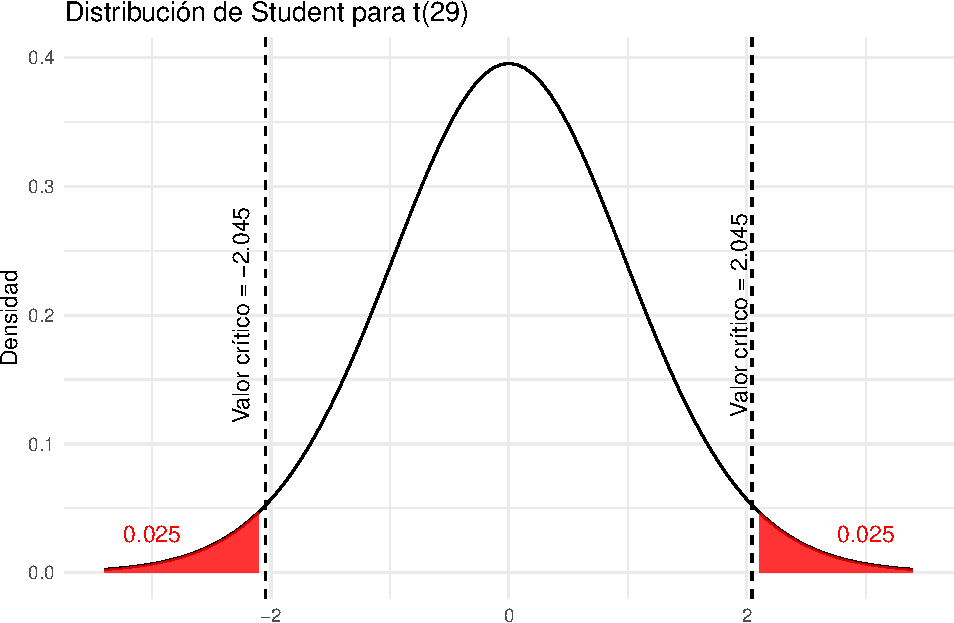
\includegraphics{tecnicas-cuantitativas_files/figure-latex/unnamed-chunk-55-1.pdf}

Al igual que en el apartado anterior, cabe recordar estos valores críticos de -2,045 y 2,045 el último paso.

Las áreas sombreadas en rojo en el gráfico anterior también se conocen como regiones de rechazo.

Estos valores críticos también se pueden encontrar en R, gracias a la función \texttt{qt\ ()}:

\begin{Shaded}
\begin{Highlighting}[]
\KeywordTok{qt}\NormalTok{(}\FloatTok{0.025}\NormalTok{, }\DataTypeTok{df =} \DecValTok{29}\NormalTok{, }\DataTypeTok{lower.tail =} \OtherTok{TRUE}\NormalTok{)}
\end{Highlighting}
\end{Shaded}

\begin{verbatim}
## [1] -2.04523
\end{verbatim}

\begin{Shaded}
\begin{Highlighting}[]
\KeywordTok{qt}\NormalTok{(}\FloatTok{0.025}\NormalTok{, }\DataTypeTok{df =} \DecValTok{29}\NormalTok{, }\DataTypeTok{lower.tail =} \OtherTok{FALSE}\NormalTok{)}
\end{Highlighting}
\end{Shaded}

\begin{verbatim}
## [1] 2.04523
\end{verbatim}

Como se ha visto en el tema sobre distribuciones de probabilidad, la función \texttt{qt\ ()} se usa para la distribución de Student (\texttt{q} significa cuantil y\texttt{t} para Student). Cabe recordar que hay otras funciones que acompañan a las diferentes distribuciones:

\begin{itemize}
\tightlist
\item
  \texttt{qnorm\ ()} para la distribución Normal
\item
  \texttt{qchisq\ ()} para la distribución Chi-cuadrado
\item
  \texttt{qf\ ()} para la distribución de Fisher
\end{itemize}

\hypertarget{conclusiuxf3n-e-interpretaciuxf3n-de-los-resultados}{%
\subsubsection{Conclusión e interpretación de los resultados}\label{conclusiuxf3n-e-interpretaciuxf3n-de-los-resultados}}

Las únicas dos posibilidades al concluir una prueba de hipótesis son:

\begin{enumerate}
\def\labelenumi{\arabic{enumi}.}
\tightlist
\item
  Rechazo de la hipótesis nula, o
\item
  No rechazo de la hipótesis nula
\end{enumerate}

En nuestro ejemplo sobre los salarios de los españoles, recordamos que hemos determinado que el:

\begin{itemize}
\tightlist
\item
  el \texttt{t-stat} es -1.369306, y
\item
  los valores críticos son -2.04523 y 2.04523
\end{itemize}

Recordemos que:

\begin{itemize}
\tightlist
\item
  el \textbf{t-stat da una indicación de cuán extrema es nuestra muestra} en comparación con la hipótesis nula
\item
  los \textbf{valores críticos son el umbral a partir del cual el t-stat se considera \emph{demasiado} extremo}
\end{itemize}

Para comparar el \texttt{t-stat} con los valores críticos de manera gráfica:

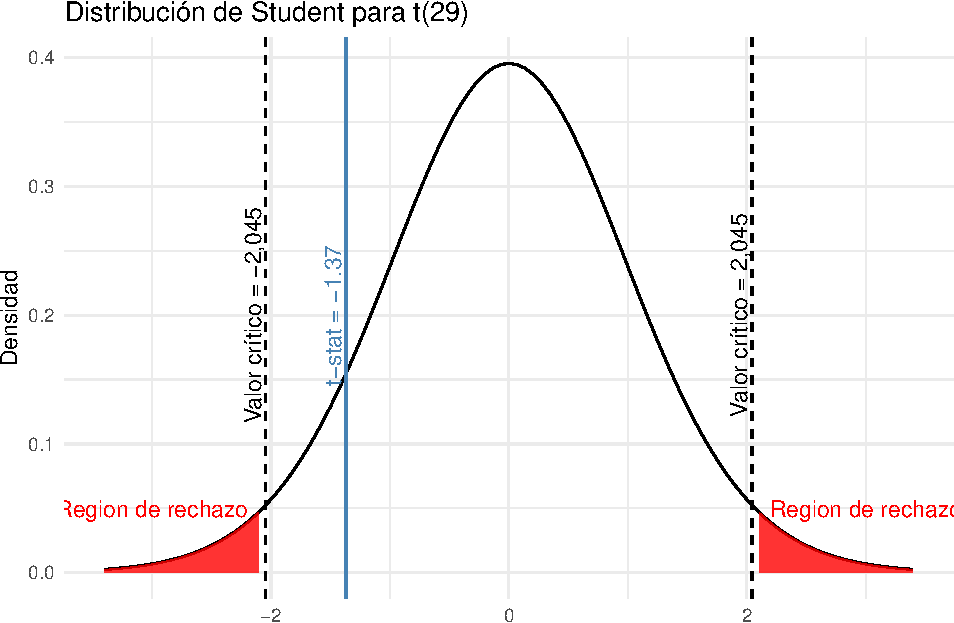
\includegraphics{tecnicas-cuantitativas_files/figure-latex/unnamed-chunk-57-1.pdf}

Los dos valores críticos forman las regiones de rechazo (las áreas sombreadas en rojo):

\begin{itemize}
\tightlist
\item
  de \(-\infty\) a -2.045, y
\item
  de 2.045 a \(\infty\)
\end{itemize}

Si el \textbf{\emph{t-stat} se encuentra dentro de una de estas regiones, rechazamos la hipótesis nula}. Por el contrario, si \textbf{t-stat \emph{no} se encuentra dentro de ninguna de las regiones, no rechazamos la hipótesis nula}.

Como podemos ver en el gráfico anterior, el \emph{t-stat} es menos extremo que el valor crítico. En conclusión, no rechazamos la hipótesis nula de que \(\mu = 1200\).

Esta es la conclusión en términos estadísticos, pero no tienen sentido sin una interpretación adecuada. Por tanto, es una buena práctica interpretar también el resultado en el contexto del problema:

\begin{quote}
Con un nivel de significancia del 5\%, no rechazamos la hipótesis de que el salario medio de los trabajadores españoles es de 1200 euros.
\end{quote}

¿Qué significa esto realmente? Dicho de otro modo:

\begin{quote}
``nosotros \emph{no rechazamos} la hipótesis nula'' y ``nosotros \emph{no rechazamos} la hipótesis de que el salario medio de los trabajadores españoles es igual a 1200 euros''. No escribimos ``\emph{aceptamos o estamos de acuerdo con} la hipótesis nula'' ni ``el salario medio de los trabajadores españoles es de 1200 euros''.
\end{quote}

En los test de hipótesis, llegamos a una conclusión sobre la población a partir de una muestra. Por tanto, siempre existe cierta incertidumbre y no podemos decir que estemos seguros al 100\% de que nuestra conclusión sea correcta.

Quizás sea el caso de que el salario medio de los trabajadores españoles sea en realidad diferente a 1200 euros, pero \textbf{no lo pudimos demostrar} con los datos disponibles. Si tuviéramos más observaciones hubiéramos rechazado la hipótesis nula (dado que todo lo demás es igual, un tamaño de muestra más grande implica un \texttt{t-stat} más extremo). O puede darse el caso de que, incluso con más observaciones, no hubiéramos rechazado la hipótesis nula porque el salario de los trabajadores españoles en realidad se acerca a los 1200 euros. Con los datos disponibles no podemos distinguir entre estas dos posibilidades. Simplemente debemos admitir que no encontramos suficiente evidencia en contra de la hipótesis de partida, pero tampoco concluimos que la media sea igual a 1200 euros.

\hypertarget{comparando-el-p-valor-con-el-nivel-de-significancia-alpha}{%
\subsection{\texorpdfstring{Comparando el \emph{p}-valor con el nivel de significancia \(\alpha\)}{Comparando el p-valor con el nivel de significancia \textbackslash alpha}}\label{comparando-el-p-valor-con-el-nivel-de-significancia-alpha}}

Este método consiste en los siguientes pasos:

\begin{enumerate}
\def\labelenumi{\arabic{enumi}.}
\tightlist
\item
  Enunciar las \textbf{hipótesis nula y alternativa}
\item
  Calcular la \textbf{estadística de prueba} (\texttt{t-stat}).
\item
  Calcular el \textbf{\emph{p}-valor}
\item
  \textbf{Concluir} e interpretar los resultados
\end{enumerate}

En este segundo método que utiliza el valor \emph{p}, los dos primeros pasos son similares a los del primer método, mientras que la interpretación de los resultados tiene algunos puntos en común.

\hypertarget{establecer-las-hipuxf3tesis}{%
\subsubsection{Establecer las hipótesis}\label{establecer-las-hipuxf3tesis}}

Las hipótesis de investigación (nula y alternativa) siguen siendo las mismas:

\begin{itemize}
\tightlist
\item
  \(H_0:\mu= 1200\)
\item
  \(H_1:\mu\ne 1200\)
\end{itemize}

\hypertarget{calcular-la-estaduxedstica-de-prueba-1}{%
\subsubsection{Calcular la estadística de prueba}\label{calcular-la-estaduxedstica-de-prueba-1}}

Cabe recordar que la fórmula del estadístico t es diferente según el tipo de prueba de hipótesis (una o dos medias, una o dos proporciones, una o dos varianzas). En nuestro caso de una sola media con varianza desconocida, tenemos que:

\[t_{obs} = \frac{\overline{x} - \mu}{\frac{s}{\sqrt{n}}} = \frac{1150 - 1200}{\frac{200}{\sqrt{30}}} = -1.369306\]

\hypertarget{calculo-del-valor-p}{%
\subsubsection{\texorpdfstring{Calculo del valor \emph{p}}{Calculo del valor p}}\label{calculo-del-valor-p}}

El \textbf{\emph{p}-valor} es la probabilidad (de 0 a 1) de observar una muestra al menos tan extrema como la que observamos si la hipótesis nula fuera cierta. Dicho de otro modo: \textbf{¿cómo de probable es la hipótesis nula?}. También se define como el nivel de significancia más pequeño para el cual los datos indican el rechazo de la hipótesis nula.

Formalmente, el valor \emph{p} es el área más allá del estadístico de prueba. Como estamos haciendo una prueba bidireccional, el valor \emph{p} es, por lo tanto, la suma del área por encima de 1,369306 y por debajo de -1,369306.

Visualmente, el valor \emph{p} es la suma de las dos áreas sombreadas en azul en la siguiente gráfica:

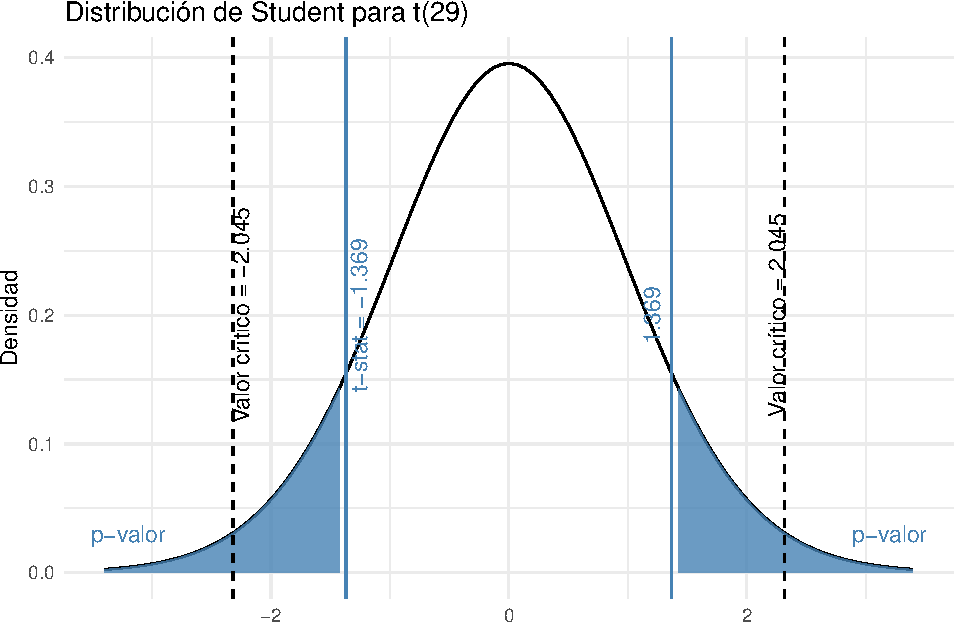
\includegraphics{tecnicas-cuantitativas_files/figure-latex/unnamed-chunk-58-1.pdf}

El valor \emph{p} se puede obtener también con tablas estadísticas o es posible calcularlo con precisión en R con la función \texttt{pt()}:

\begin{Shaded}
\begin{Highlighting}[]
\NormalTok{p_val <-}\StringTok{ }\KeywordTok{pt}\NormalTok{(}\OperatorTok{-}\FloatTok{1.369306}\NormalTok{, }\DataTypeTok{df =} \DecValTok{29}\NormalTok{, }\DataTypeTok{lower.tail =} \OtherTok{TRUE}\NormalTok{) }\OperatorTok{+}\StringTok{ }\KeywordTok{pt}\NormalTok{(}\FloatTok{1.369306}\NormalTok{, }\DataTypeTok{df =} \DecValTok{29}\NormalTok{, }\DataTypeTok{lower.tail =} \OtherTok{FALSE}\NormalTok{)}
\NormalTok{p_val}
\end{Highlighting}
\end{Shaded}

\begin{verbatim}
## [1] 0.1814156
\end{verbatim}

\begin{Shaded}
\begin{Highlighting}[]
\CommentTok{# Que es lo mismo que...}
\NormalTok{p_val <-}\StringTok{ }\DecValTok{2} \OperatorTok{*}\StringTok{ }\KeywordTok{pt}\NormalTok{(}\FloatTok{1.369306}\NormalTok{, }\DataTypeTok{df =} \DecValTok{29}\NormalTok{, }\DataTypeTok{lower.tail =} \OtherTok{FALSE}\NormalTok{)}
\NormalTok{p_val}
\end{Highlighting}
\end{Shaded}

\begin{verbatim}
## [1] 0.1814156
\end{verbatim}

El valor \emph{p} es 0.1814, que indica que hay un 18.14\% de probabilidad de observar una muestra al menos tan extrema como la observada si el hipótesis nula eran verdaderas. Esto ya nos da una pista sobre si nuestro t-stat es demasiado extremo o no (y, por lo tanto, si nuestra hipótesis nula es probable o no).

Como la función \texttt{qt()} para encontrar el valor crítico, usamos \texttt{pt()} para encontrar el valor \emph{p} porque la distribución subyacente es la distribución de Student. En otros casos se utilizarían las funciones \texttt{pnorm\ ()}, \texttt{pchisq\ ()} y \texttt{pf\ ()} para las otras distribuciones mencionadas anteriormente (Normal, Chi-cuadrado y Fisher).

\hypertarget{concluir-e-interpretar-los-resultados}{%
\subsubsection{Concluir e interpretar los resultados}\label{concluir-e-interpretar-los-resultados}}

Finalmente, hay que comparar el valor \emph{p} que acabamos de calcular con el nivel de significancia \(\alpha\). Como para todas las pruebas estadísticas:

\begin{itemize}
\tightlist
\item
  Si el \textbf{\emph{p}-valor es menor} que \(\alpha\) (p-valor\(<0.05\)), entonces \(H_0\) es poco probable \(\rightarrow\) \textbf{rechazamos} la hipótesis nula.
\item
  Si el \textbf{\emph{p}-valor es mayor que o igual} a \(\alpha\) (\emph{p}-valor \(\ge 0.05\)), entonces \(H_0\) es probable \(\rightarrow\) \textbf{no podemos rechazar} la hipótesis nula.
\end{itemize}

No importa si tomamos en consideración el \emph{p}-valor exacto (es decir, 0.1814) o el acotado (0.05 \textless{}\emph{p}-valor \textless0.10), es mayor que 0.05, entonces no rechazamos la hipótesis nula. En el contexto del problema, no rechazamos la hipótesis nula de que el salario medio de los trabajadores españoles es igual a 1200 euros.

El resultado obtenido ha sido el mismo que en el primer método. Evidentemente, debería dar lo mismo si se usan los mismos datos y con el mismo nivel de significancia.

\hypertarget{comparaciuxf3n-del-paruxe1metro-objetivo-con-el-intervalo-de-confianza}{%
\subsection{Comparación del parámetro objetivo con el intervalo de confianza}\label{comparaciuxf3n-del-paruxe1metro-objetivo-con-el-intervalo-de-confianza}}

Este método consiste en calcular primero el intervalo de confianza y comparar sobre éste el parámetro objetivo (el parámetro bajo la hipótesis nula). Podemos distinguir tres pasos:

\begin{enumerate}
\def\labelenumi{\arabic{enumi}.}
\tightlist
\item
  Enunciar las \textbf{hipótesis nula y alternativa}
\item
  Calcular el \textbf{intervalo de confianza}
\item
  \textbf{Concluir} e interpretar los resultados
\end{enumerate}

También se pueden apreciar varias similitudes con los métodos anteriores.

\hypertarget{enunciar-las-hipuxf3tesis}{%
\subsubsection{Enunciar las hipótesis}\label{enunciar-las-hipuxf3tesis}}

Nuevamente, las hipótesis nula y alternativa siguen siendo las mismas:

\begin{itemize}
\tightlist
\item
  \(H_0:\mu = 1200\)
\item
  \(H_1:\mu\ne 1200\)
\end{itemize}

\hypertarget{calcular-el-intervalo-de-confianza}{%
\subsubsection{Calcular el intervalo de confianza}\label{calcular-el-intervalo-de-confianza}}

Al igual que los test de hipótesis, los intervalos de confianza son una herramienta bien conocida en la estadística inferencial. El \textbf{intervalo de confianza} es un procedimiento de estimación que produce un \textbf{intervalo que contiene el parámetro verdadero con una cierta probabilidad}.

De la misma manera que existe una fórmula para cada tipo de prueba de hipótesis al calcular las estadísticas de la prueba, existe una fórmula para cada tipo de intervalo de confianza. La fórmula para calcular un intervalo de confianza en una media \(\mu\) (con varianza poblacional desconocida):
\[
(1-\alpha)\% \text{ IC para } \mu=\overline{x}\pm t_{\alpha/2, n - 1}\frac{s}{\sqrt{n}}
\]
donde \(t_{\alpha/2, n-1}\) se encuentra en la tabla de distribución de Student o se puede calcular con R (y es similar al valor crítico encontrado en el primer método).

Dados nuestros datos y con \(\alpha= 0.05\), tenemos que:
\[
\begin{aligned}
 95\%\text{ IC para } \mu 
    &= \overline{x} \pm t_{\alpha/2, n - 1} \frac{s}{\sqrt{n}} \\
    &= 1150 \pm 2.045 \frac{200}{\sqrt{30}} \\
    &= [1075,33; 1224,67]
\end{aligned}
\]

El intervalo de confianza del 95\% para \(\mu\) es {[}1075,33; 1224,67{]} euros. \textbf{¿Qué significa este intervalo de confianza del 95\%? }

Sabemos que este procedimiento de estimación tiene una probabilidad del 95\% de producir un intervalo que contenga la media verdadera \(\mu\). En otras palabras, \textbf{si construimos muchos intervalos de confianza} (con diferentes muestras del mismo tamaño), \textbf{el 95\% de ellos incluirá la media de la población} (el verdadero parámetro). Del mismo modo el 5\% de estos intervalos de confianza no cubrirán la media real.

Si desea disminuir este último porcentaje, puede disminuir el nivel de significancia (por ejemplo \(\alpha= 0.01\)). En igualdad de condiciones, esto disminuirá el rango del intervalo de confianza y, por lo tanto, aumentará la probabilidad de que incluya el parámetro verdadero.

\hypertarget{conclusiuxf3n-e-interpretaciuxf3n-de-los-resultados-1}{%
\subsubsection{Conclusión e interpretación de los resultados}\label{conclusiuxf3n-e-interpretaciuxf3n-de-los-resultados-1}}

Finalmente, hay comparar el intervalo de confianza con el valor del parámetro objetivo (el valor cuestionado por la hipótesis nula):

\begin{itemize}
\tightlist
\item
  Si el \textbf{intervalo de confianza no incluye} el valor hipotético, \(H_0\) es poco probable \(\rightarrow\) \textbf{rechazamos} la hipótesis nula.
\item
  Si el \textbf{intervalo de confianza incluye} el valor hipotético, \(H_0\) es probable \(\rightarrow\), \textbf{no rechazamos} la hipótesis nula
\end{itemize}

En nuestro ejemplo:

\begin{itemize}
\tightlist
\item
  el valor hipotético es 1200 (desde \(H_0:\mu= 1200\))
\item
  1200 se incluye en el intervalo de confianza del 95\%, ya que va de 1075,33 a 1224,67 euros
\item
  Entonces \textbf{no rechazamos} la hipótesis nula de que el salario medio de los trabajadores españoles sea de 1200 euros.
\end{itemize}

Por supuesto, la conclusión es equivalente a la que se había llegado por los otros dos métodos. Esto debe ser así, ya que usamos los mismos datos y el mismo nivel de significancia \(\alpha\) para los tres métodos.

\hypertarget{test-de-hipuxf3tesis-en-r-cuxe1lculo-e-informes}{%
\section{Test de hipótesis en R: cálculo e informes}\label{test-de-hipuxf3tesis-en-r-cuxe1lculo-e-informes}}

\hypertarget{un-ejemplo-sobre-brecha-salarial-entre-guxe9neros}{%
\section{Un ejemplo sobre brecha salarial entre géneros}\label{un-ejemplo-sobre-brecha-salarial-entre-guxe9neros}}

\hypertarget{anova}{%
\section{ANOVA}\label{anova}}

\hypertarget{algunas-consideraciones-finales}{%
\section{Algunas consideraciones finales}\label{algunas-consideraciones-finales}}

\hypertarget{cuando-no-se-necesita-inferencia}{%
\subsection{¿Cuando no se necesita inferencia?}\label{cuando-no-se-necesita-inferencia}}

Hemos analizado varios ejemplos sobre cómo realizar inferencias estadísticas: realización de test de hipótesis y construcción de intervalos de confianza. Antes de empezar a realizar un experimento, siempre es necesario realizar un análisis exploratorio de los datos. Este primer vistazo siempre puede ayudar a intuir sobre lo que los métodos estadísticos como los intervalos de confianza y las pruebas de hipótesis pueden decirnos (y lo que no pueden). En los apartados anteriores hemos querido explicar cómo funciona la inferencia pero no nos hemos preguntado si era realmente necesaria.

Consideremos un ejemplo. Supongamos que estamos interesados en la siguiente pregunta: De \emph{todos} los vuelos que salen de un aeropuerto de la ciudad de Nueva York, ¿los vuelos de Hawaiian Airlines están en el aire por más tiempo que los vuelos de Alaska Airlines? Además, supongamos que los vuelos de 2013 son una muestra representativa de todos esos vuelos. Entonces podemos usar el dataframe \texttt{flights} disponible en el paquete \texttt{nycflights13} para responder nuestra pregunta. Filtremos este dataframe para incluir solo a Hawaiian y Alaska Airlines usando sus códigos de ``operador'' ``HA'' y ``AS'':

\begin{Shaded}
\begin{Highlighting}[]
\KeywordTok{library}\NormalTok{(tidyverse)}
\KeywordTok{library}\NormalTok{(nycflights13)}
\NormalTok{flights_sample <-}\StringTok{ }\NormalTok{flights }\OperatorTok\StringTok{ }
\StringTok{  }\KeywordTok{filter}\NormalTok{(carrier }\OperatorTok\StringTok{ }\KeywordTok{c}\NormalTok{(}\StringTok{"HA"}\NormalTok{, }\StringTok{"AS"}\NormalTok{))}
\end{Highlighting}
\end{Shaded}

Hay dos posibles métodos de inferencia estadística que podríamos utilizar para responder a estas preguntas. Primero, podríamos construir un intervalo de confianza del 95\% para la diferencia en las medias poblacionales \(\mu_{HA}-\mu_{AS}\), donde \(\mu_{HA}\) es el tiempo de vuelo medio de todos los vuelos de Hawaiian Airlines y \(\mu_{AS}\) es el tiempo medio de vuelo de los vuelos de Alaska Airlines. Luego podríamos verificar si la totalidad del intervalo es mayor que 0, sugiriendo que \(\mu_{HA} - \mu_{AS}> 0\), o, en otras palabras, sugiriendo que \(\mu_{HA}> \mu_{AS}\). En segundo lugar, podríamos realizar una prueba de hipótesis de la hipótesis nula \(H_0:\mu_{HA} - \mu_{AS} = 0\) frente a la hipótesis alternativa \(H_A:\mu_{HA}-\mu_{AS}>0\).

Construyamos primero una visualización exploratoria como acabamos de sugerir. Dado que \texttt{air\_time} es numérico y \texttt{carrier} es categórico, un diagrama de caja (\emph{boxplot}) puede mostrar la relación entre estas dos variables (ver la Figura \ref{fig:ha-as-flights-boxplot}).

\begin{Shaded}
\begin{Highlighting}[]
\KeywordTok{ggplot}\NormalTok{(}\DataTypeTok{data =}\NormalTok{ flights_sample, }\DataTypeTok{mapping =} \KeywordTok{aes}\NormalTok{(}\DataTypeTok{x =}\NormalTok{ carrier, }\DataTypeTok{y =}\NormalTok{ air_time)) }\OperatorTok{+}
\StringTok{  }\KeywordTok{geom_boxplot}\NormalTok{() }\OperatorTok{+}
\StringTok{  }\KeywordTok{labs}\NormalTok{(}\DataTypeTok{x =} \StringTok{"Carrier"}\NormalTok{, }\DataTypeTok{y =} \StringTok{"Air Time"}\NormalTok{)}
\end{Highlighting}
\end{Shaded}

\begin{figure}
\centering
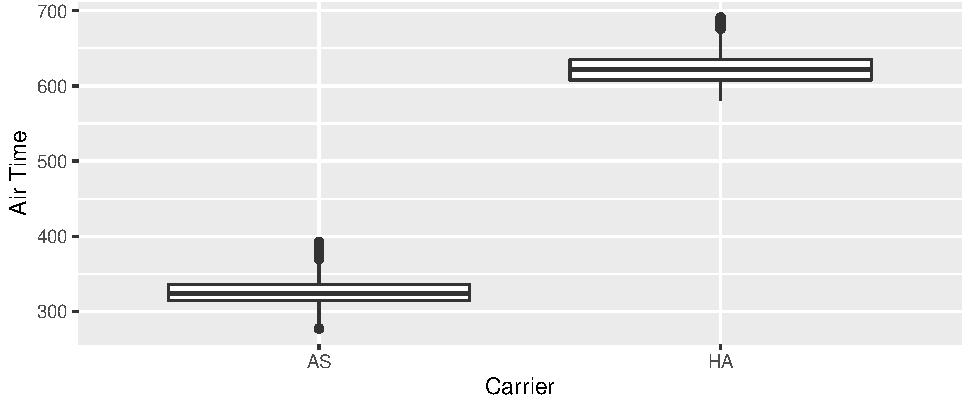
\includegraphics{tecnicas-cuantitativas_files/figure-latex/ha-as-flights-boxplot-1.pdf}
\caption{\label{fig:ha-as-flights-boxplot}Air time for Hawaiian and Alaska Airlines flights departing NYC in 2013.}
\end{figure}

Esto es lo que nos gusta llamar momentos en los que ``no se necesita un doctorado en estadística''. No es necesario ser un experto en estadísticas para saber que Alaska Airlines y Hawaiian Airlines tienen horarios aéreos \emph{significativamente} diferentes. ¡Los dos diagramas de caja ni siquiera se superponen! La construcción de un intervalo de confianza o la realización de una prueba de hipótesis, francamente, no proporcionaría mucha más información que la Figura \ref{fig:ha-as-flights-boxplot}.

Investiguemos por qué observamos una diferencia tan clara entre estas dos aerolíneas que utilizan la manipulación de datos. Primero agrupemos por las filas de \texttt{vuelos\_muestra} no solo por\texttt{transportista} sino también por destino \texttt{dest}. Posteriormente, calcularemos dos estadísticas resumidas: el número de observaciones usando \texttt{n\ ()} y el tiempo medio de transmisión:

\begin{Shaded}
\begin{Highlighting}[]
\NormalTok{flights_sample }\OperatorTok\StringTok{ }
\StringTok{  }\KeywordTok{group_by}\NormalTok{(carrier, dest) }\OperatorTok\StringTok{ }
\StringTok{  }\KeywordTok{summarize}\NormalTok{(}\DataTypeTok{n =} \KeywordTok{n}\NormalTok{(), }\DataTypeTok{mean_time =} \KeywordTok{mean}\NormalTok{(air_time, }\DataTypeTok{na.rm =} \OtherTok{TRUE}\NormalTok{))}
\end{Highlighting}
\end{Shaded}

\begin{verbatim}
## # A tibble: 2 x 4
## # Groups:   carrier [2]
##   carrier dest      n mean_time
##   <chr>   <chr> <int>     <dbl>
## 1 AS      SEA     714      326.
## 2 HA      HNL     342      623.
\end{verbatim}

Resulta que desde la ciudad de Nueva York en 2013, Alaska solo voló a ``SEA'' (Seattle) desde la ciudad de Nueva York (NYC) mientras que Hawaiian solo voló a ``HNL'' (Honolulu) desde Nueva York. Dada la clara diferencia en la distancia entre la ciudad de Nueva York y Seattle y la ciudad de Nueva York a Honolulu, no es sorprendente que observemos tiempos de vuelo tan diferentes (\_ estadísticamente significativamente diferentes\_, de hecho) en los vuelos.

Este es un claro ejemplo de que no es necesario hacer nada más que un simple análisis exploratorio de datos utilizando visualización de datos y estadísticas descriptivas para llegar a una conclusión adecuada. Por lo tanto, es recomendable empezar siempre por realizar un análisis exploratorio con estadísticas descriptivas antes de aplicar inferencia estadística.

\hypertarget{problemas-con-los-p-valores}{%
\subsection{Problemas con los p-valores}\label{problemas-con-los-p-valores}}

Además de los muchos malentendidos comunes sobre las pruebas de hipótesis y los valores de \(p\) que hemos comentado al explicar la interpretación de las pruebas de hipótesis, otra consecuencia desafortunada del uso ampliado de los valores de \(p\) y las pruebas de hipótesis es un fenómeno conocido como ``p-hacking'', que es es el acto de ``seleccionar'' sólo los resultados que son ``estadísticamente significativos'' y descartar los que no lo son, aunque sea a expensas de las ideas científicas. Hay muchos artículos escritos recientemente sobre malentendidos y problemas con los valores de \(p\). Le recomendamos que consulte algunos de ellos:

\begin{enumerate}
\def\labelenumi{\arabic{enumi}.}
\tightlist
\item
  \href{https://en.wikipedia.org/wiki/Misunderstandings_of_p-values}{Malentendidos de los valores de \(p\)}
\item
  \href{https://www.vox.com/science-and-health/2017/7/31/16021654/p-\%20valores-significación-estadística-redefinir-0005}{Qué debate más nerd sobre los valores de \(p\) sobre la ciencia y cómo solucionarlo}
\item
  \href{https://www.nature.com/news/statisticians-issue-warning-over-misuse-of-p-values-1.19503}{Los estadísticos emiten una advertencia sobre el uso indebido de los valores de \(p\)}
\item
  \href{https://fivethirtyeight.com/features/you-cant-trust-what-you-read-about-nutrition/}{No puede confiar en lo que lee sobre nutrición}
\item
  \href{http://www.fharrell.com/post/pval-litany/}{Una letanía de problemas con valores p}
\end{enumerate}

Tales problemas se estaban volviendo tan recurrentes que la Asociación Estadounidense de Estadística (ASA) emitió una declaración en 2016 titulada, \href{https://www.amstat.org/asa/files/pdfs/P-ValueStatement.pdf}{``Declaración de la ASA sobre la importancia estadística y los valores de \(p\)''} con seis principios subyacentes al uso e interpretación adecuados de los valores de \(p\). La ASA publicó esta guía sobre los valores de \(p\) para mejorar la conducta y la interpretación de la ciencia cuantitativa y para informar el creciente énfasis en la reproducibilidad de la investigación científica.

Quizás el uso de intervalos de confianza para la inferencia estadística permita evitar ciertos malentendidos. Sin embargo, en muchos campos todavía se usan exclusivamente valores de \(p\) para la inferencia estadística y esta es una razón para incluirlos en este texto.

\hypertarget{ejercicios-2}{%
\section{Ejercicios}\label{ejercicios-2}}

\hypertarget{distribuciuxf3n-binomial}{%
\subsection{Distribución Binomial}\label{distribuciuxf3n-binomial}}

En nuestro municipio hay 500 hombres de la misma edad y con buena salud. Según las estadísticas actuales, la probabilidad de que estas personas vivan 30 años o más es de 2/3. Hay que hallar las probabilidades de que dentro de esos 30 años vivan

\begin{enumerate}
\def\labelenumi{\arabic{enumi}.}
\tightlist
\item
  Los 500 hombres.
\item
  Al menos 300 de ellos.
\item
  200 hombres
\end{enumerate}

\hypertarget{distribuciuxf3n-normal}{%
\subsection{Distribución Normal}\label{distribuciuxf3n-normal}}

El ayuntamiento consume una media de 80 \(kWh/hab/a\), con una desviación estándard de 14\(kWh/hab/a\). Hay que calcular:

\begin{enumerate}
\def\labelenumi{\arabic{enumi}.}
\tightlist
\item
  La probabilidad de que este año hagan falta entre 75 y 90 (\(p(75 \leqslant x \leqslant 90)\)).
\item
  La probabilidad de que hagan falta 75 o menos (\(p(75 \leqslant x\)).
\item
  Describid en un párrafo alguna variable municipal que se pueda ajustar a una distribución normal y haced la comprobación.
\end{enumerate}

\hypertarget{el-muestreo-estaduxedstico}{%
\chapter{El muestreo estadístico}\label{el-muestreo-estaduxedstico}}

Some \emph{significant} applications are demonstrated in this chapter.

\hypertarget{example-one}{%
\section{Example one}\label{example-one}}

\hypertarget{example-two}{%
\section{Example two}\label{example-two}}

\hypertarget{regresiones}{%
\chapter{Regresiones}\label{regresiones}}

We have finished a nice book.

\hypertarget{estaduxedstica-multivariante}{%
\chapter{Estadística multivariante}\label{estaduxedstica-multivariante}}

We have finished a nice book.

  \bibliography{book.bib,packages.bib}

\end{document}
